\documentclass{theme/uniprthesis}

%%%%%%%%%%%Some Extra Packages%%%%%%%%%%%
\usepackage[italian]{babel}		% To have Italina names in Sections, Figures, Chapters etc.
\usepackage{todonotes}			% To ease the revision

\usepackage{blindtext} 			% Dummy Text - remove

\usepackage{hyperref}			% link library
\usepackage{listings}
\usepackage{color}
\usepackage{xcolor}
\usepackage{float}% http://ctan.org/pkg/float
%%%%%%%%%%%%%%%%%%%%%%%%%%%%%%%%%


%%%%%%%%%%%%Custom%%%%%%%%%%%%%%%%%%%%%
% inline code
\definecolor{codebackground}{HTML}{ededeb}
\newcommand{\inlinecode}[1]{\colorbox{codebackground}{\textcolor{red}{#1}}}
\newcommand{\noteStyle}[1]{\textit{#1}}

\hypersetup{
    colorlinks=true,
    linkcolor=blue,
    filecolor=magenta,      
    urlcolor=cyan,
    pdfpagemode=FullScreen,
    }

\urlstyle{same}
%%%%%%%%%%%%%%%%%%%%%%%%%%%%%%%%%


%%%%% THESIS / TITLE PAGE INFORMATION
% Everybody needs to complete the following:

\title{Titolo in Italiano}
\author{Dennis Turco}
\advisor{Prof.\ Roberto Alfieri}
\college{Dipartimento di Scienze Matematiche, Fisiche e Informatiche}
\degree{Corso di Laurea [Triennale in Informatica]}
\degreeyears{2020--2023}


% Not mandatory fields
\newcommand{\subTitle}{Titolo in Inglese} %Subtitle, usually the english version of the title

%\newcommand{\advisorSecond}{Prof. Nome2 Cognome2} % For multiple (up to 4) advisors -- if this is not present then also the remaining ones are automatically omitted
%\newcommand{\advisorThird}{Dott. Nome3 Cognome3} % For multiple (up to 4) advisors -- if this is not present then also the remaining ones are automatically omitted
%\newcommand{\advisorFourth}{Dott. Nome4 Cognome4} % For multiple (up to 4) advisors

\newcommand{\coadvisor}{Prof.\ co-Nome co-Cognome} %For multiple (up to 4) coadvisors -- if this is not present then also the remaining ones are automatically omitted
\newcommand{\coadvisorSecond}{Prof.\ co-Nome2 co-Cognome2} % For multiple (up to 4) coadvisors -- if this is not present then also the remaining ones are automatically omitted
%\newcommand{\coadvisorThird}{Dott. co-Nome3 co-Cognome3} % For multiple (up to 4) coadvisors -- if this is not present then also the remaining ones are automatically omitted
%\newcommand{\coadvisorFourth}{Dott. co-Nome4 co-Cognome4} % For multiple (up to 4) coadvisors

\begin{document}

\maketitle

%%%% La dedica
% \newpage
% \thispagestyle{empty}
% \null\vspace{\stretch{1}}
% \begin{flushright}
% 	\textit{Dedica}
% \end{flushright}
% \vspace{\stretch{3}}\null
% \newpage

%%%% Gli indici
\pagestyle{plain}
\pagenumbering{roman}
\tableofcontents
%
\listoffigures    %Commentare se non vi sono Immagini
%\listofalgorithms %Commentare se non vi sono Algoritmi
\lstlistoflistings
%\listoftables     %Commentare se non vi sono Tabelle
%
%
%
%%%% La prefazione
\chapter*{Introduzione}\label{chapter:introduzione} %Se si cambia il Titolo cambiare anche la riga successiva così che appia corretto nell'indice
\addcontentsline{toc}{chapter}{Introduzione} %Per far apparire Introduzione nell'indice (Il nome deve rispecchiare quello del chapter)
\pagenumbering{arabic} % Settaggio numerazione normale
Nel seguente elaborato tratterò una relazione relativa al progetto di tirocinio svolto 
presso un'azienda software house “ISolutions” di Noceto.
\\ \\
Il progetto si concentra sulla creazione di una piattaforma di e-learning per la 
gestione del processo di OnBoarding aziendale.\ L'obiettivo è di fornire ai nuovi 
dipendenti un'esperienza guidata, strutturata e personalizzata attraverso la 
piattaforma web. 
\\ \\
Attualmente, l'azienda gestisce tra 20 e 30 processi di OnBoarding dei nuovi 
dipendenti ogni anno, grazie al personale HR, utilizzando un foglio di calcolo Excel 
per la gestione dei dati e del completamento dei vari task.\ Tuttavia questo metodo si 
basa su un funzionamento manuale di aggiornamento dei task completati dai vari 
dipendenti e richiede una supervisione umana costante, il che lo rende inefficiente e 
non scalabile.\ Inoltre, le informazioni raccolte attraverso il modulo post-OnBoarding 
non sono sempre esaustive e dettagliate.\ A causa dell'espansione dell'azienda, 
questo sistema sta diventando sempre più inefficiente e rischioso.\ Per questo motivo 
risulta importante l'implementazione di un software dedicato al processo di 
OnBoarding dei dipendenti, con lo scopo di garantire una riduzione del rischio di 
errori e di migliorare l'esperienza generale.\ Inoltre, il software deve permettere di 
automatizzare alcune attività ripetitive, liberando tempo prezioso per il team HR, che 
potrà concentrarsi su attività di maggiore valore aggiunto per l'azienda.\ Infine, il 
nuovo sistema di OnBoarding ha la necessità di consentire l'acquisizione e 
l'archiviazione in maniera più sicura e organizzata dei dati dei dipendenti, 
rispettando le normative sulla privacy e semplificando le attività di audit interno.
\\ \\
Il processo di OnBoarding avrà una durata di circa un mese per uno sviluppatore 
junior e due settimane per uno sviluppatore senior.\ La piattaforma guiderà i nuovi 
dipendenti attraverso i vari task previsti in modo strutturato e personalizzato, 
fornendo loro gli strumenti necessari per acquisire le conoscenze e le competenze 
richieste per il loro ruolo. \\
Inoltre, la piattaforma fornirà un modulo per la raccolta di feedback post-OnBoarding. 
Il modulo sarà strutturato in modo da raccogliere informazioni dettagliate e utili per 
migliorare continuamente il processo di OnBoarding. Questo feedback sarà utilizzato 
per aggiornare e migliorare costantemente la piattaforma. \\ 
Infine, poiché l'azienda è certificata ISO 9001 (certificazione della qualità), la 
piattaforma fornirà un'ulteriore valutazione del processo di OnBoarding. Dopo che il 
dipendente ha completato il processo, verrà chiesto di esprimere un giudizio 
attraverso un modulo dedicato. Ciò permetterà all'azienda di comprendere se il 
processo di OnBoarding sta funzionando correttamente e se ci sono aree che 
possono essere migliorate. \\ 
In sintesi, la piattaforma di e-learning per la gestione del processo di OnBoarding 
aziendale rappresenta un'importante innovazione per l'azienda.\ Grazie alla sua 
efficienza e scalabilità, la piattaforma migliorerà l'esperienza del dipendente e ridurrà 
il carico di lavoro del personale HR.\ Inoltre, la raccolta di feedback dettagliati post-OnBoarding
 e la valutazione attraverso il modulo dedicato forniranno all'azienda le 
informazioni necessarie per migliorare costantemente il processo di OnBoarding.
\\ \\
Il processo pricincipale di OnBoarding aziendale deve prevedere le seguenti fasi.
\begin{itemize}
    \item Introduzione (\textasciitilde{10} tasks);
    \item Setup della work station (\textasciitilde{20} tasks);
    \item Documentazione, sia amministrativa che tecnica (\textasciitilde{30} tasks);
    \item Video introduttivi, tecnici e orientati ai prodotti sviluppati (\textasciitilde{10} tasks);
    \item Overview dell'organizzazione aziendale e degli strumenti utilizzati (\textasciitilde{10} tasks);
    \item Hands On degli applicativi aziendali (\textasciitilde{20} tasks);
    \item Formazione sui principali linguaggi di programmazione utilizzati (\textasciitilde{20} tasks);
    \item Overview struttura codice delle soluzioni software (\textasciitilde{10} tasks);
    \item Test finale con revisione e valutazione.
\end{itemize}
Sono previsti inoltre alcuni step preliminari, in carico al team HR, per la predispozione di quanto 
necessario (creazione utenza, preparazione pc etc\dots), e una fase finale di 
retrospettiva per raccogliere feedback riguardo il processo dal neo assunto.\ 
\\ \\
Alcune desiderate del progetto:
\begin{itemize}
    \item Integrazione autenticazione con modulo di login e gestione livelli di autorizzazione;
    \item Pannello amministrativo per il team HR per gestire (creazione, modifica, eliminazione) dei vari tasks;
    \item Tracciamento tempo impiegato sui vari task e reportistica per team HR;\
    \item Possibilità di avviare, sospendere e saltare un task;
    \item Integrazione fase finale di test, revisione e valutazione.
\end{itemize}
Il progetto di creazione della piattaforma di e-learning per la gestione del processo di
OnBoarding aziendale è stato realizzato come web application .NET MVC 6.0
utilizzando molteplici tecnologie e linguaggi di programmazione tra cui: C\#, HTML, 
Css, Javascript, SQL.

%
%%%% I Capitoli di Contenuto	
\pagestyle{fancy}
\chapter{Le caratteristiche dell'OnBoarding}\label{chapter:caratteristiche_onboarding}
Il processo di OnBoarding, sebbene possa inizialmente apparire come una fase apparentemente semplice e marginale, 
riveste in realtà un'importanza cruciale nel contesto dell'integrazione dei nuovi membri nell'organico di iSolutions.\
Come precedentemente introdotto nella sezione iniziale di questo elaborato,
il processo di OnBoarding è tipicamente strutturato su un periodo di circa un mese, ma è fondamentale sottolineare che 
la sua durata può variare considerevolmente da un dipendente all'altro.\ Questo periodo iniziale di integrazione, 
che potrebbe superficialmente sembrare un'appendice, svolge in realtà una serie di funzioni di rilevanza vitale.
\\ \\
È importante notare che il processo di OnBoarding viene coordinato e gestito con grande cura da un team HR altamente specializzato.\ 
Questo team opera con precisione e attenzione ai dettagli per garantire una transizione efficace e senza intoppi per i nuovi arrivati.\ 
La sua importanza ricade con lo scopo di offrire una garanzia di un'ottimale integrazione dei nuovi dipendenti nell'ambiente aziendale.
\\ \\
Risulta evidente che il processo di OnBoarding richiede un approccio attento e uniforme da parte di tutto il personale aziendale.\ 
Questa necessità è strettamente correlata alla complessità delle operazioni svolte da iSolutions e alla diversità dei numerosi 
strumenti e tecnologie che l'azienda utilizza, compresi quelli di natura proprietaria.\ Questi strumenti rivestono un ruolo 
centrale sia nella gestione che nell'analisi dei dati aziendali e nei processi operativi nel loro complesso.\ 
Inoltre, essi giocano un ruolo significativo nella consegna di servizi di alta qualità ai clienti dell'azienda.
\\ \\
In questo contesto, diventa chiaro che un nuovo membro del team deve affrontare l'obiettivo di familiarizzarsi 
con tali tecnologie e procedure aziendali.\ Questo obiettivo viene raggiunto attraverso il processo di OnBoarding, 
che svolge il ruolo di guida nella presentazione di tutte le conoscenze iniziali necessarie per lavorare in modo produttivo 
all'interno del sistema aziendale. Durante questa fase, i nuovi arrivati avranno l'opportunità di acquisire familiarità con 
gli strumenti, i linguaggi, le convenzioni aziendali e i protocolli che sono essenziali per contribuire al successo e 
all'efficienza dell'azienda.
\\ \\
Pertanto, il processo di OnBoarding, lungi dall'essere una mera formalità, rappresenta un elemento fondamentale per il successo 
e il corretto funzionamento di iSolutions e deve essere affrontato con la massima serietà e impegno da parte di tutti i suoi attori.
\\ \\
Il processo di OnBoarding è un'attività complessa che si pone diversi obiettivi, 
e pertanto è strutturato in diverse sezioni con l'intento di fornire ai nuovi 
dipendenti una conoscenza iniziale completa.\ Le sezioni principali del processo di OnBoarding all'interno dell'azienda iSolutions si suddividono in:
\begin{itemize}
    \item \textbf{Introduction and account setup}: I task all'interno di questo sistema sono incentrati sull'integrazione del dipendente 
    nell'azienda e includono l'attivazione dell'account aziendale, come l'accesso alla casella di posta e la configurazione di una VPN per 
    il lavoro remoto, insieme ad altre attività connesse;
    \item \textbf{Work station setup}: I task all'interno di questo processo mirano a guidare il dipendente nell'installazione di tutti 
    i programmi necessari per svolgere il lavoro in azienda;
    \item \textbf{Documentation}: Si tratta di una collezione di documenti che il nuovo dipendente deve leggere al fine di familiarizzarsi 
    con le dinamiche e il regolamento aziendale;
    \item \textbf{Video}: Questa sezione raccoglie un insieme di video guide da visualizzare con l'obiettivo di assistere il dipendente 
    nella configurazione di alcuni sistemi e di fornirgli una comprensione del loro funzionamento;
    \item \textbf{Company tools \& organization}: I task all'interno hanno lo scopo di consentire al dipendente di acquisire familiarità con 
    l'organizzazione aziendale tramite la visione di documenti come organigrammi, documenti organizzativi e gli strumenti più utilizzati;
    \item \textbf{Hands On}: I task all'interno sono interamente dedicati all'esecuzione di test specifici all'interno di programmi 
    proprietari, al fine di acquisire familiarità con gli strumenti necessari per il lavoro futuro del dipendente;
    \item \textbf{SQL}: I task all'interno hanno l'obiettivo di far eseguire al dipendente query in linguaggio SQL per 
    consentirgli di acquisire familiarità con la struttura del database interno;
    \item \textbf{Coding}: I task interni sono progettati per orientare il dipendente nel mondo della programmazione interna 
    e nello sviluppo dei servizi aziendali utilizzando diversi linguaggi e sistemi interni;
    \item \textbf{Agile}: I task all'interno riguardano l'introduzione del dipendente al sistema Agile aziendale, 
    con un'ampia panoramica sulla metodologia; 
\end{itemize}
%
Al momento, come precedentemente accennato, il processo di OnBoarding non fa uso di un sistema automatizzato; 
al contrario, è gestito attraverso un semplice foglio Excel. Questo foglio è consultato dai dipendenti interessati 
e viene modificato manualmente quando il dipendente termina le relative attività interne da parte del personale HR incaricato.\ 
Tuttavia, questo approccio presenta alcune limitazioni.\ 
Innanzitutto, non permette di raccogliere e organizzare dati statistici derivati dall'uso del processo.\ 
In secondo luogo, non offre la possibilità agli utenti di interagire direttamente con il sistema.

\begin{figure}[H]
	\centering
	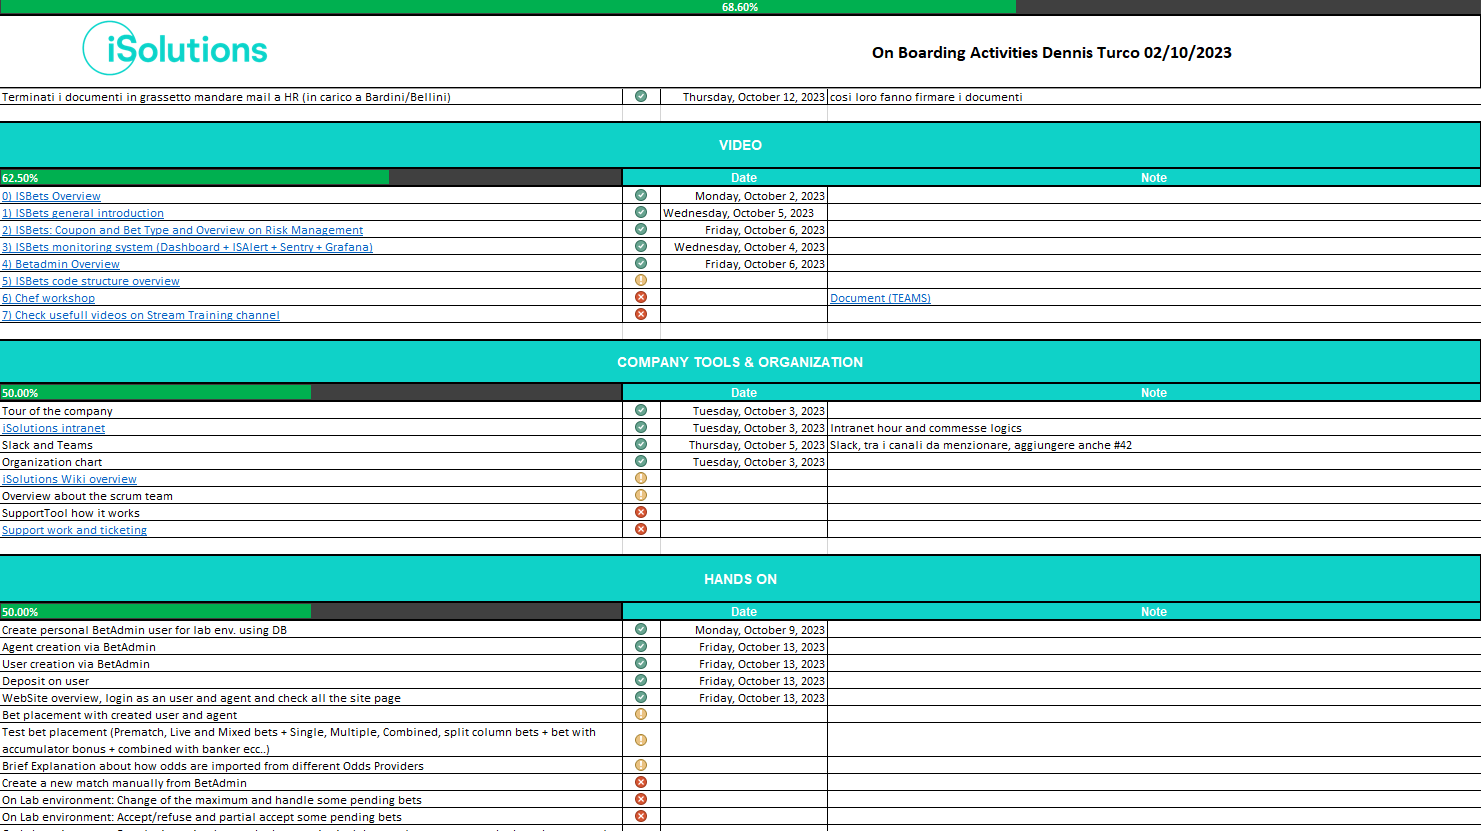
\includegraphics[width=\textwidth]{img/OnBoardingExcel.png}
	\caption{struttura del file excel di OnBoarding}
	\label{fig:OnBoardingExcel}
\end{figure}

Ciò significa che, con l'attuale modalità, manca l'opportunità di ottenere una visione dettagliata e sistematica dell'andamento del processo di OnBoarding, 
impedendo all'azienda di identificare potenziali aree di miglioramento o di misurare l'efficacia del processo stesso.\ 
Inoltre, l'assenza di un'interazione diretta con il sistema può ostacolare la comunicazione e la partecipazione attiva dei dipendenti nel corso 
del processo, rendendo l'integrazione meno fluida e coinvolgente.
\\ \\
Pertanto, esiste un evidente margine per l'implementazione di un sistema automatizzato di OnBoarding che non solo semplificherebbe 
la gestione, ma consentirebbe anche la raccolta e l'analisi di dati utili per ottimizzare il processo e coinvolgere in modo più 
attivo i dipendenti coinvolti.

\chapter{Le tecnologie utilizzate}\label{chapter:formattazione}
%
Il progetto di creazione della piattaforma di e-learning per la gestione del processo di 
OnBoarding aziendale è stato realizzato utilizzando molteplici tecnologie, servizi e linguaggi:
%
\section{Tecnologie e Servizi}\label{sec:cap_sec_subsec}
\begin{enumerate}
    \item ASP.NET MVC 6.0;
    \item Autenticazione;
    \item GitHub;
    \item Git;
\end{enumerate}
\subsection{ASP.NET MVC 6.0}\label{sec:cap_sec_subsec}
ASP.NET Core MVC è un ricco framework creato da Microsoft per la creazione di applicazioni web e API 
utilizzando il modello di progettazione Model-View-Controller.
\begin{itemize}
    \item Model: Il back-end che contiene tutta la logica dei dati;
    \item View: interfaccia utente front-end o grafica (GUI);
    \item Controller: Il ``cervello'' dell'applicazione che controlla come vengono visualizzati i dati.
\end{itemize}
\subsection{Autenticazione con ``Identity''}\label{sec:cap_sec_subsec}
Siccome il progetto in questione riguarda la creazione di una piattaforma web, è stato necessario
implementare il servizio di Autenticazione attraverso il framework ASP.NET Core Identity, al
fine di otterenere non soltanto la possibilità di permettere le azioni di login e registrazione da parte degli utenti, ma
anche di farlo ottenendo una sicurezza dei dati sensibili. 
\\ \\
In particolare la forma di Autenticazione utilizzata nella piattaforma è una ``Forms Authentication'', ovvero, è quel tipo di
autenticazione nella quale l'utente deve fornire le proprie credenziali attraverso un form dedicato. 
\\ \\
ASP.NET Core Identity è un API che supporta funzionalità di login lato UI.\ Gestisce utenti,
password, dati del profilo, ruoli, email di conferma e molto altro. \\
In particolare, gli utenti possono creare un account con le informazioni di accesso memorizzate in Identity 
o possono utilizzare un provider di accesso esterno (es. Facebook, Google, ecc\dots ).
\\ \\
\textit{Nota:} L'algoritmo utilizzato dal servizio Identity per criptare le password è PBKDF2 (Password-Based Key Derivation Function 2):
\begin{lstlisting}[style=cs_style, caption=algoritmo di hashing per criptare le password usato dal servizio Identity]
public static string HashPassword(string password)
{
    byte[] salt;
    byte[] bytes;
    if (password == null)
    {
        throw new ArgumentNullException("password");
    }
    using (Rfc2898DeriveBytes rfc2898DeriveByte = new Rfc2898DeriveBytes(password, 16, 1000))
    {
        salt = rfc2898DeriveByte.Salt;
        bytes = rfc2898DeriveByte.GetBytes(32);
    }
    byte[] numArray = new byte[49];
    Buffer.BlockCopy(salt, 0, numArray, 1, 16);
    Buffer.BlockCopy(bytes, 0, numArray, 17, 32);
    return Convert.ToBase64String(numArray);
}
    \end{lstlisting}


\subsection{GitHub}\label{sec:cap_sec_subsec}
Il progetto durante il suo sviluppo è stato salvato in un'apposità repository privata
su GitHub. \\
GitHub è stato fondamentale per tenere una traccia storica di tutte le
modifiche apportate nel corso del tempo, in risposta all'esecuzione dei vari task assegnati. \\
Esso non si è limitato ad essere un semplice strumento a d'uso esclusivamente
individuale, ma ha permesso la condivisione del lavoro sia con il tutor 
aziendale che con il resto del personale.
\subsection{Git}\label{sec:cap_sec_subsec}
In parallelo all'utilizzo di GitHub è stato impiegato il software di controllo di versione Git 
con l'obbiettivo di agevolare l'aggiornamento dei file del progetto dalla workspace locale verso 
la repository privata che ospita il progetto, tramite appositi commit.
\section{Linguaggi}\label{sec:cap_sec_subsec}
\begin{enumerate}
    \item SQL;
    \item C\#;
    \item HTML, CSS, JavaScript;
\end{enumerate}
%
\subsection{SQL}\label{sec:cap_sec_subsec}
Il linguaggio SQL è stato utilizzato per 
la creazione del database del sito web.\ Il database contiene tutte le informazioni 
necessarie per la corretta gestione della piattaforma, tra cui i dati relativi agli utenti 
registrati, ai corsi e alle categorie dei corsi.
%
\subsection{C\#}\label{sec:cap_sec_subsec}
Il linguaggio C\# è stato utilizzato per la gestione della parte back-end del sito, 
creando un dialogo tra le informazioni contenute nel database e l'interfaccia utente.\
L'accesso ai dati del database tramite il linguaggio C\# è stato possibile grazie 
al framework ``Dapper'', che consente di eseguire interrogazioni in modo efficace ed 
efficiente.\ In questo modo, il sito è più responsivo anche in caso di grandi quantità di 
dati da gestire, eliminando elementi come le procedure, che risultano meno 
manutenibili e più complicate da gestire a causa di una complicazione del codice nella 
parte back-end per il loro utilizzo. 
\\ \\
Il linguaggio C\# è stato anche utilizzato per la 
gestione degli eventi, la navigazione tra le pagine e i controlli di vario genere.\
L'utilizzo di molteplici 
tecnologie ha permesso di ottenere un prodotto completo e funzionale, in grado di 
soddisfare le esigenze dell'azienda e dei nuovi dipendenti.
%
\subsection{HTML, CSS, JavaScript}\label{sec:cap_sec_subsec}
Per la gestione dell'interfaccia utente, sono stati utilizzati il linguaggio HTML, il 
linguaggio CSS e il linguaggio JavaScript.\ Il linguaggio HTML è stato utilizzato per la 
creazione della struttura del sito, il linguaggio CSS per la gestione dello stile e il 
linguaggio JavaScript per la gestione degli eventi.
\chapter{Il progetto e il suo sviluppo}\label{chapter:formattazione}
%
\section{Tree Structure}\label{sec:cap_sec_subsec}

La tree structure (figura~\ref{fig:treeStructure}) del progetto si suddivide in diverse sottocartelle.\\ 
Di seguito, commenterò solo le cartelle che risultano rilevanti per la discussione:
\begin{itemize}
	\item \textbf{wwwroot}: Contiene file per la gestione della parte grafica, 
	in particolare, include, in apposite sottocartelle, i file HTML, CSS, JavaScript e le immagini utilizzate. 
	\item \textbf{Areas}: Contiene i file generati automaticamente dal framework ASP.NET Core Identity.
	\item \textbf{Controllers}: Contiene i file scritti in linguaggio C\# che svolgono un 
	ruolo fondamentale nella gestione delle richieste HTTP e nell'orchestrazione 
	delle azioni dell'applicazione.\ Questi file fungono da punto di ingresso per 
	le richieste HTTP, coordinano le azioni dell'applicazione, manipolano i dati e 
	restituiscono risposte HTTP appropriate.
	\item \textbf{Migrations}: Contiene i file in linguaggio C\# relativi alle migrations.
	\item \textbf{Models}: Contiene solo file C\#, che vengono utilizzati per rappresentare 
	le entità e i dati all'interno dell'applicazione, contribuendo così a mantenere il 
	codice organizzato e coeso.
	\item \textbf{Query}: Contiene esclusivamente file SQL, il cui utilizzo è ormai superato.\ 
	I file contenuti in questa cartella non influenzano l'esecuzione della piattaforma.\
	In particolare, questi file erano stati originariamente utilizzati per conservare le procedure, 
	ma sono state successivamente rimpiazzate dall'uso del framework Dapper. 
	\item \textbf{View}: Contiene numerosi file di tipo CSHTML, organizzati in diverse 
	sottocartelle.\ Questi file sono responsabili di come i dati vengono presentati 
	all'utente, gestendo l'aspetto, la struttura e l'interfaccia utente dell'applicazione.
\end{itemize}
%
\begin{figure}[H]
	\centering
	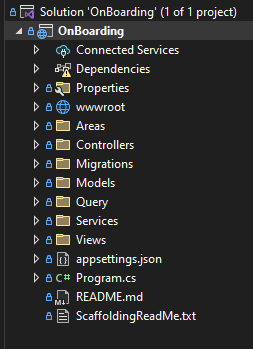
\includegraphics[width=0.5\textwidth]{img/treeStructure.png}
	\caption{tree structure del progetto}
	\label{fig:treeStructure}
\end{figure}
%
\section{Database}\label{sec:cap_sec_subsec}
Una parte sostanziale del lavoro impiegato per portare a compimento il
progetto si è concentrata in modo dettagliato sulla creazione del database,
ritenuto elemento cruciale per assicurare il pieno funzionamento della
piattaforma. 
\\ \\ 
La creazione del database è stata articolata in diverse fasi chiave:
\begin{itemize}
	\item Progettazione della struttura del database, un processo attentamente studiato.
	\item Scrittura del database in linguaggio SQL, una tappa essenziale per l'implementazione della struttura.
	\item Implementazione delle interrogazioni al database nella sezione di back-end,
	      facendo uso della libreria Dapper.
\end{itemize}
\textit{Nota}: il database è stato creato e gestito unicamente in locale per questioni di semplicità e per
l'esecuzione di test sulla correttezza della struttura e dell'implementazione del database stesso.
%
\subsection{Progettazione}
La fase di progettazione (figura~\ref{fig:progettazione_database}) del database ha occupato un ruolo
fondamentale nel corso di questo processo, coinvolgendo un'analisi costante e
una riflessione profonda. L'obbiettivo principale è stato quello di plasmare un
database estremamente completo, in grado di soddisfare appieno le esigenze
della piattaforma di e-learning, ponendosi lo scopo aggiuntivo di:
\begin{itemize}
	\item Migliorare la leggibilità del database;
	\item Rendere più agevole la manutenzione;
	\item Fornire ampie possibilità di estensione del sistema.
\end{itemize}
\begin{figure}[H]
	\centering
	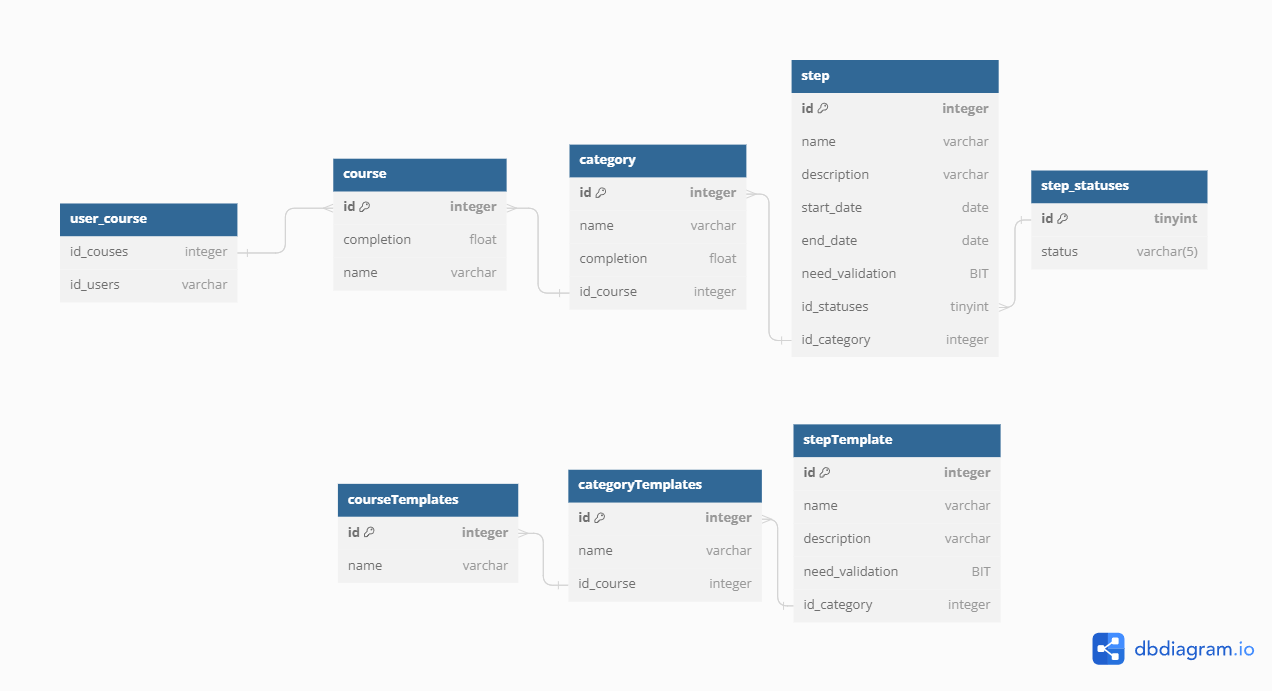
\includegraphics[width=\textwidth]{img/progettazione_database.png}
	\caption[progettazione del database]{la progettazione mostrata non tiene traccia delle tabelle utente, perchè vengono
	gestite automaticamente dal progetto .NET grazie al servizio di autenticazione già
	incluso (libreria \inlinecode{Microsoft.AspNet.Identity.EntityFramework;}).}
	\label{fig:progettazione_database}
\end{figure}
%
Si noti, inoltre, che non è stato creato un collegamento tra le tabelle “*Templates” con il resto del tabelle
perchè esse vengono gestite in maniera del tutto indipendente con le altre informazioni e relazioni presenti.
\begin{figure}[H]
	\centering
	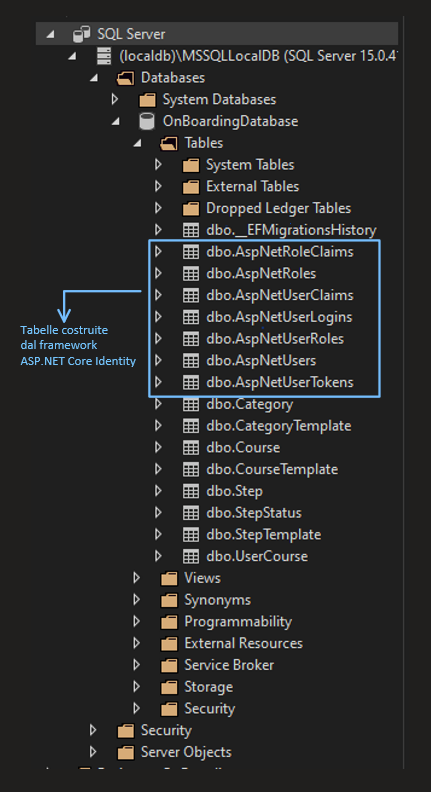
\includegraphics[width=0.5\textwidth]{img/TreeStructureDatabase.png}
	\caption{tree structure del database}
	\label{fig:TreeStructureDatabase}
\end{figure}
%
\subsection{Scrittura nel linguaggio SQL}
Il risultato finale di questa fase è possibile visualizzarlo nella sezione appendice di questo elaborato (appendice~\ref{appendice-database}).\\ 
\textit{Nota}: non sono riportate le tabelle generate dal servizio di Autenticazione, perchè gestite automaticamente dalla
libreria a disposizione.
%
\subsection{Interrogazioni al Database}
Inizialmente, le interrogazioni al database erano state sviluppate attraverso
stored procedure.\ Tra i numerosi vantaggi proposti, l'idea principale era ottenere:
\begin{itemize}
	\item Riutilizzo del codice;
	\item Semplificazione della manutenzione;
	\item Prestazioni migliorate;
\end{itemize}
Tuttavia, durante lo sviluppo dell'applicativo, grazie al suggerimento di alcuni membri
dell'azienda, si è preferito sostituire le procedure con interrogazioni dirette dal codice
tramite il framework Dapper, al fine di poter migliorare:
\begin{itemize}
	\item Prestazioni in termini di tempo;
	\item Semplificare il debugging del codice;
	\item Centrallizzare l'intera logica in un unico posto.
\end{itemize}
All'interno della piattaforma si possono distinguere 3 macro categorie di interrogazioni per:
\begin{itemize}
	\item Inserimento dei dati riguardanti:
		\begin{itemize}
			\item utenti
			\item corsi;
			\item categorie (sotto gruppo dei corsi);
			\item step (sotto gruppo delle categorie);
			\item corsi template;
			\item categorie template (sotto gruppo dei corsi template);
			\item step template (sotto gruppo delle categorie template).
		\end{itemize}
	\item Eliminazione dei dati riguardanti:
		\begin{itemize}
			\item utenti
			\item corsi;
			\item categorie (sotto gruppo dei corsi);
			\item step (sotto gruppo delle categorie);
			\item corsi template;
			\item categorie template (sotto gruppo dei corsi template);
			\item step template (sotto gruppo delle categorie template).
		\end{itemize}
	\item Lettura dei dati per permettere di ottenere tutte le informazioni necessarie
		per la generazione corretta della pagina dinamica dato un determinato utente
		connesso;
\end{itemize}
%
\section{Scrittura del codice C\#}\label{sec:cap_sec_subsec}
La parte del codice back-end rappresenta il nucleo vitale dell'intero progetto, 
che ne garantisce il corretto funzionamento. Questa componente è stata completamente 
sviluppata utilizzando il linguaggio di programmazione C\#.
\\ \\
L'obbiettivo principale è stato garantire una gestione efficiente del database
direttamente attraverso il codice, sfruttando appieno le potenzialità del
framework Dapper. \\ 
Utilizzando C\# e il framework Dapper, è stato possibile
realizzare un corretto collegamento tra dati e utenti.\ Questo ha reso
possibile la generazione dinamica e accurata delle pagine web, consentendo
un'esperienza utente ottimale. 
\\ \\ 
Per eseguire delle query al database è
stato necessario creare una connessione dal codice C\# al database attraverso
la libreria \inlinecode{Microsoft.Data.SqlClient;}
%
\begin{lstlisting}[style=cs_style, caption=classe per ottenere la stringa di connessione per il collegamento al database]
using Microsoft.Data.SqlClient;
using Microsoft.EntityFrameworkCore;

namespace OnBoarding.Services
{
	public class ConnectionService
	private SqlConnection _connection = new SqlConnection();
	private SqlCommand _command = new SqlCommand();

	public static IConfiguration? Configuration { get; set; }

	public string GetconnectionString()
	{
		var builder = new ConfigurationBuilder().SetBasePath(Directory.GetCurrentDirectory()).AddJsonFile("appsettings.json");

		Configuration = builder.Build();
		return Configuration.GetConnectionString("ApplicationDBContextConnection");
	}


	public SqlConnection GetConnection() 
	{
		return _connection;
	}

	public SqlCommand GetCommand()
	{
		return _command;
	}

	}
}
\end{lstlisting}
%
In questo modo, una volta che è stata stabilita una connessione, 
è stato reso possibile il processo di scrittura di query. A titolo esemplificativo, si può menzionare 
la query nella funzione denominata ``GetCourses'' presente all'interno del file ``CourseManager.cs''.\ Questa query, 
quando viene fornito l'ID dell'utente come input, ha lo scopo principale di recuperare e restituire 
l'insieme completo dei corsi associati all'utente specificato.
%
\begin{lstlisting}[style=cs_style, caption=esempio funzione per l'esecuzione di una query da codice tramite il framework Dapper]
public List<CourseModel> GetCourses(string userid)
{
	using (_connection = new SqlConnection(connectionService.GetconnectionString()))
	{
		_connection.Open();

		string sql = 
			@"SELECT DISTINCT Course.* 
			FROM Course, AspNetUsers, UserCourse 
			WHERE UserCourse.UserId = @userId     
			AND UserCourse.CourseId = Course.Id";
		var coursesList = _connection.Query<CourseModel>(sql, new { userId = userid }).ToList();

		_connection.Close();

		return coursesList;
	}
} 
\end{lstlisting}
%
Si osserva che ciascun utente può essere associato a più corsi, 
stabilendo così una relazione uno a molti.\ Pertanto, è fondamentale 
che il valore restituito dalla funzione sia di tipo \inlinecode{List\textless CourseModel\textgreater}, 
in quanto questa struttura dati può contenere più di un corso associato a 
un utente specifico.\ Inoltre, grazie all'uso di Dapper, è possibile effettuare 
un'interrogazione al database mediante una stringa appositamente creata 
(come mostrato nelle righe 7\--11 del codice).\ Successivamente, è possibile 
ottenere il risultato dell'interrogazione corrispondente al parametro ``userid'' 
fornito alla funzione e al campo ``userId'' nella tabella ``Course'' (riga 12 del codice).
\\
Notare che siccome la funzione ritorna in questo caso una lista, il risultato della query
dovrà essere convertito in una collezione di oggetti dello stesso tipo (attraverso alla funzione \inlinecode{ToList()}).
%
\\ \\
%
Un punto di particolare rilevanza che merita menzione è rappresentato dallo sviluppo di una classe denominata 
``StatisticsController.cs''.\ Il suo scopo principale consiste nell'elaborare in modo esaustivo e dettagliato tutte 
le statistiche associate a un utente specifico.\ Questa classe si avvale della sofisticata libreria \inlinecode{ClosedXML.Excel;} 
per generare dati statistici in formato csv~\ref{fig:exportToExcel}, inerenti al completamento dei corsi che sono stati non solo avviati, ma anche portati a 
termine dall'utente in questione.\ È essenziale sottolineare che questa funzionalità è rigorosamente riservata agli 
utenti che detengono il privilegiato ruolo di ``Admin''.
%
\begin{figure}[H]
	\centering
	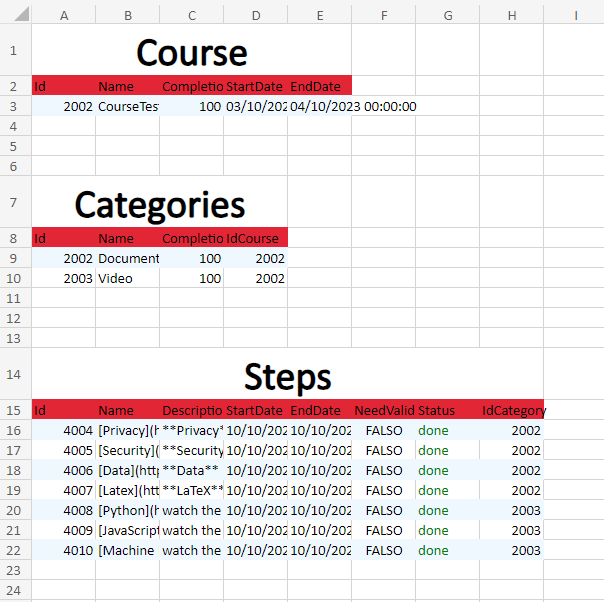
\includegraphics[width=\textwidth]{img/exportToExcel.png}
	\caption{esempio di conversione in csv}
	\label{fig:exportToExcel}
\end{figure}
%
\begin{lstlisting}[style=cs_style, caption=funzione utilizzata per l'esportazione in file exel]
[HttpGet]
[Authorize(Roles = "Admin")]
public IActionResult ExportToExcel(int id)
{
	using (var workbook = new XLWorkbook())
	{
		CourseModel course = _courseManager.GetCourseByID(id);

		var ws = workbook.Worksheets.Add(course.Name); // Sheet Name
		int i = 1;

		/////////////////////////////////////// Course
		ws.Range($"A{i}:E{i}").Merge();
		ws.Cell(i, 1).Value = "Course";
		ws.Cell(i, 1).Style.Font.Bold = true;
		ws.Cell(i, 1).Style.Alignment.Horizontal = XLAlignmentHorizontalValues.Center;
		ws.Cell(i, 1).Style.Font.FontSize = 30;

		// Header
		i++;
		ws.Cell(i, 1).Value = "Id";
		ws.Cell(i, 2).Value = "Name";
		ws.Cell(i, 3).Value = "Completion";
		ws.Cell(i, 4).Value = "StartDate";
		ws.Cell(i, 5).Value = "EndDate";
		ws.Range($"A{i}:E{i}").Style.Fill.BackgroundColor = XLColor.Alizarin;

		// Body
		i++;
		ws.Cell(i, 1).Value = course.Id;
		ws.Cell(i, 2).Value = course.Name;
		ws.Cell(i, 3).Value = course.Completion;
		if (course.StartDate != DateTime.MinValue) ws.Cell(i, 4).Value = course.StartDate.ToString();
		else { ws.Cell(i, 4).Value = "NULL"; ws.Cell(i, 4).Style.Font.FontColor = XLColor.Red; }
		if (course.EndDate != DateTime.MinValue) ws.Cell(i, 5).Value = course.EndDate.ToString();
		else { ws.Cell(i, 5).Value = "NULL"; ws.Cell(i, 5).Style.Font.FontColor = XLColor.Red; }
		ws.Range($"A{i}:E{i}").Style.Fill.BackgroundColor = XLColor.AliceBlue;
		i += 1;

		// ...
		// Stesso procedimento appena descritto per i Corsi, viene fatto
		// per le Categorie e gli Step 
		
		using (var stream = new MemoryStream())
		{
			workbook.SaveAs(stream);
			var content = stream.ToArray();
			return File(
					content,
					"application/vnd.openxmlformats-officedocument-spreadsheetml.sheet",
					course.Name + ".csv"
				);
		}
	}
}
\end{lstlisting}
%
Un aspetto di notevole rilevanza è stato il processo di gestione dei dati statistici all'interno della pagina denominata 
``/Views/Statistics/Index.cshtml''.\ Questa pagina ha una funzione fondamentale poiché consente agli admin di visualizzare 
l'insieme completo delle statistiche.\ Ciò è reso possibile grazie alla capacità di ordinare agevolmente le informazioni 
presenti all'interno delle tabelle.\ Questa caratteristica permette agli utenti di organizzare i dati in base alle loro 
specifiche esigenze e criteri di ricerca.
\\
Inoltre, per rendere l'esperienza ancora più interattiva e informativa, è stata inclusa una sezione di codice dedicata 
direttamente all'interno della pagina stessa, utilizzando il tag \inlinecode{\textless script\textgreater\ \dots \textless /script\textgreater}. Questo approccio ha 
consentito di incorporare efficacemente dei grafici che offrono una rappresentazione visiva dei dati statistici.\ 
Questi grafici sono stati sviluppati in modo da offrire quattro diverse visualizzazioni, ognuna delle quali fornisce un'analisi 
dettagliata dei dati statistici, permettendo agli utenti di comprendere meglio i pattern e le tendenze sottostanti.
\begin{itemize}
	\item due grafici a barre;
	\begin{itemize}
		\item Il primo rappresenta la somma totale dei corsi suddivisi per stato di completamento (done, running, todo);
		\item Il secondo rappresenta il numero di corsi completati in relazione al mese dell'anno.
	\end{itemize}
	\item due grafici a torta;
	\begin{itemize}
		\item Il primo rappresenta il tempo medio di completamento necessario per terminare uno specifico corso, suddiviso per corso;
		\item Il secondo rappresenta il tempo medio di completamento necessario per teminare uno specifico corso, suddiviso per utenti.
	\end{itemize}
\end{itemize}
L'implementazione del codice per la creazione dei grafici è stata effettuata mediante l'uso del linguaggio di programmazione JavaScript.\ 
Un aspetto interessante da sottolineare è che i dati numerici necessari per la creazione dei grafici non sono stati ottenuti direttamente 
tramite il codice JavaScript, ma sono stati acquisiti attraverso apposite funzioni getter scritte in codice C\#.\ 
Questo approccio è stato adottato per garantire l'accuratezza e la coerenza dei dati, nonché per sfruttare le funzionalità di gestione 
dei dati messe a disposizione dal linguaggio C\#.\
In sostanza, il processo è stato il seguente: il codice JavaScript si è interfacciato con il codice C\# attraverso apposite funzioni getter, 
ottenendo così i dati numerici necessari per alimentare i grafici.\
\begin{lstlisting}[style=javascript_style, caption=esempio sezione codice Javascript per la creazione di un grafico a barre per la rappresentazione dei dati]
<script>
	// ...
	
	// -------------------------------- BAR CHART
    var xValues = ["To Do", "Running", "Done"];
    var yValues = [@todo, @running, @done, 0];
    var barColors = ["red", "#e5e600", "green"];

    new Chart("BarChart", {
        type: "bar",
        data: {
            labels: xValues,
            datasets: [{
                backgroundColor: barColors,
                data: yValues
            }]
        },
        options: {
            legend: { display: false },
            title: {
                display: false,
                text: ""
            }
        }
    });

	// ...
</script>
\end{lstlisting}
%
\begin{figure}[H]
	\centering
	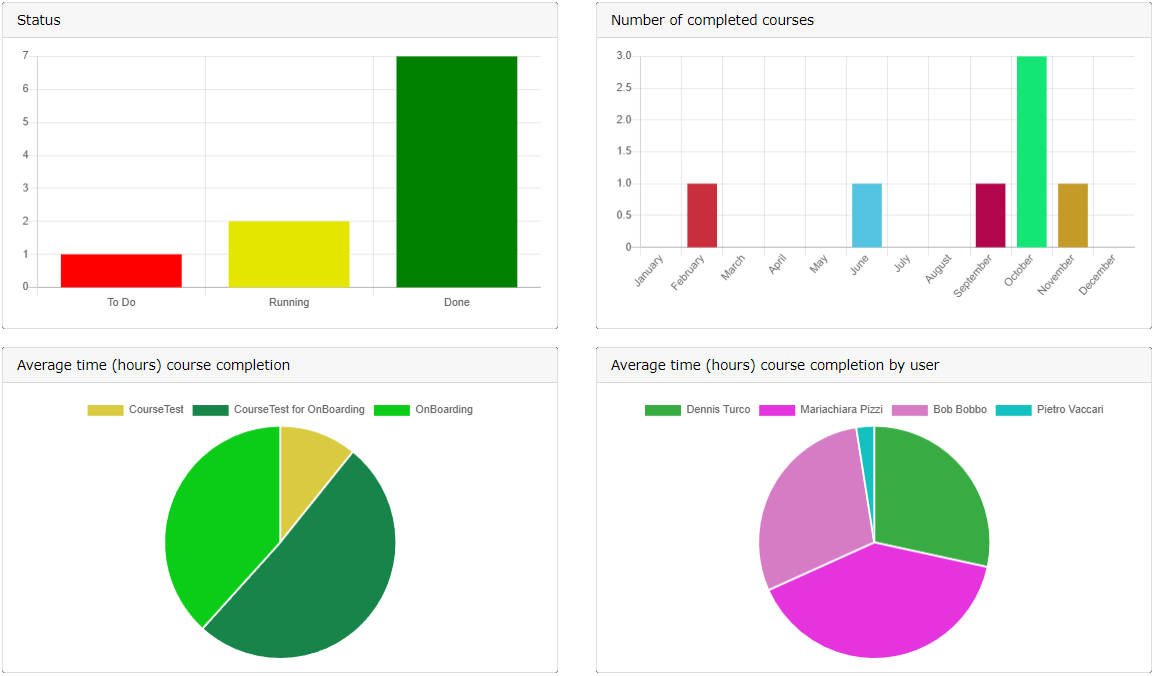
\includegraphics[width=\textwidth]{img/charts.png}
	\caption{grafici per la visualizzazione dei dati}
	\label{fig:charts}
\end{figure}
%
\section{Layout della piattaforma}\label{sec:cap_sec_subsec}
Nonostante alcune limitazioni evidenti nel design della piattaforma, che potrebbe essere descritto come non completamente moderno e, 
in alcuni aspetti, forse un po' troppo minimalista, il layout della piattaforma è stato progettato e realizzato con l'obiettivo di 
creare un servizio che sia estremamente intuitivo e facile da utilizzare, sia per gli utenti 
che per gli amministratori responsabili della gestione degli accessi e del progresso degli utenti 
durante il loro percorso nell'esperienza.\ Grazie a questa attenzione all'usabilità, 
è stato possibile assicurarsi che l'intera esperienza sia accessibile e fruibile in modo agevole 
e soddisfacente per tutti i suoi utilizzatori.
\\ \\

\begin{figure}[H]
	\centering
	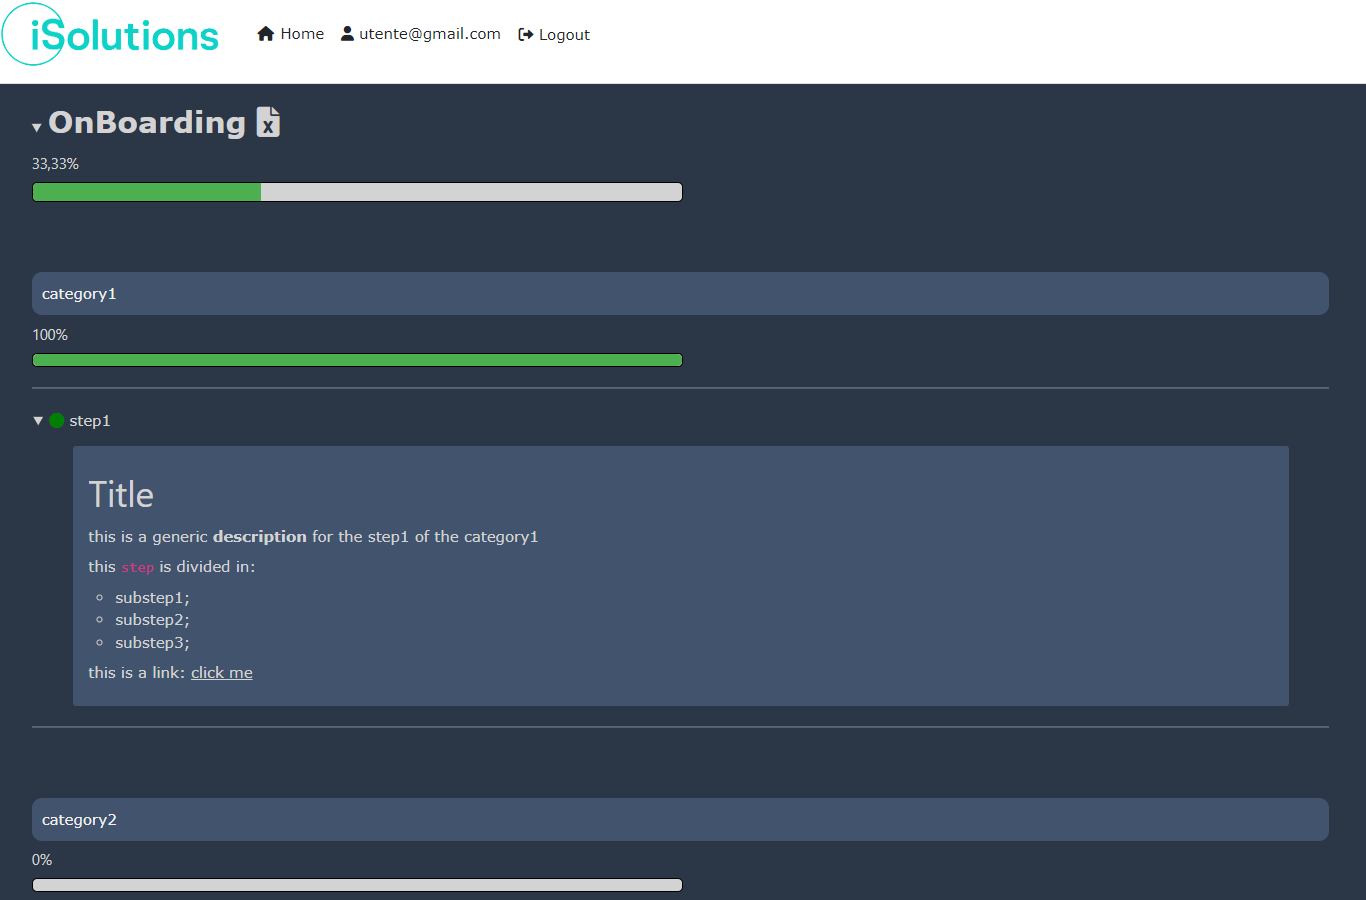
\includegraphics[width=0.9\linewidth]{img/UserView.png}
	\caption{visualizzazione lato utente}
	\label{fig:UserView}
\end{figure}

Un'aggiunta di notevole interesse dal punto di vista del layout è stata l'integrazione 
della visualizzazione in sintassi Markdown (figura~\ref{fig:markdown}) (grazie all'utilizzo dei tag \inlinecode{\textless md-block\textgreater} e \inlinecode{\textless md-span\textgreater}).\
Questa nuova funzionalità mira a migliorare 
l'esperienza dell'utente durante la visualizzazione delle descrizioni delle informazioni 
testuali presenti all'interno dei corsi.\ L'obiettivo è ottenere una visualizzazione che 
favorisca una maggiore leggibilità delle informazioni e permetta l'integrazione di 
elementi come immagini, titoli, sottotitoli e molto altro all'interno delle descrizioni 
dei task.\ Questo offre maggiore flessibilità e personalizzazione agli amministratori 
incaricati della creazione dei corsi.


% \begin{figure}[H]
% 	\centering
% 	\begin{subfigure}{0.3\textwidth}
% 		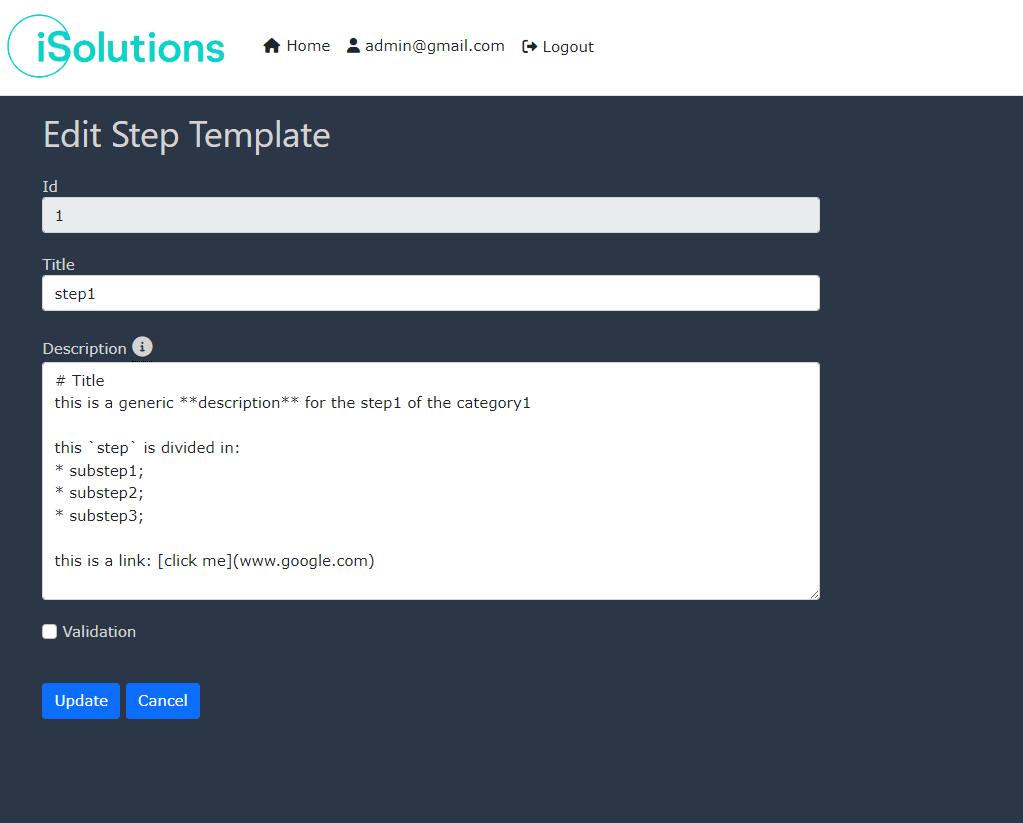
\includegraphics[width=\textwidth]{img/markdown_p1.png}
% 		\caption{scrittura in Markdown}
% 	\end{subfigure}%
% 	\begin{subfigure}{0.3\textwidth}
% 		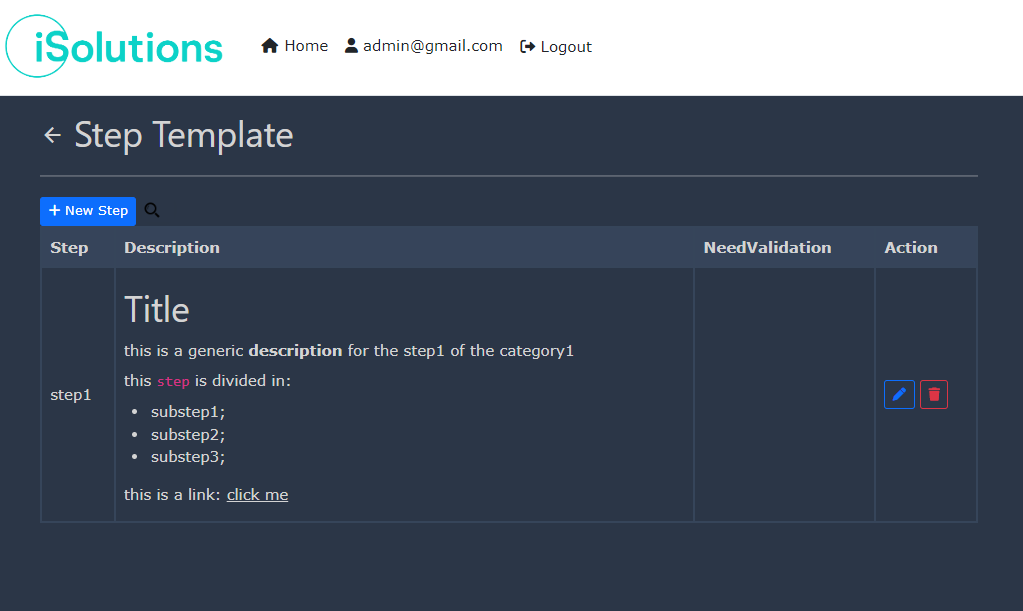
\includegraphics[width=\textwidth]{img/markdown_pt2.png}
% 		\caption{visualizzazione in Markdown}
% 	\end{subfigure}
% 	\caption{esempio di scrittura e visualizzazione in Markdown}
% 	\label{fig:markdown}
% \end{figure}

\begin{figure}[H]
	\centering
	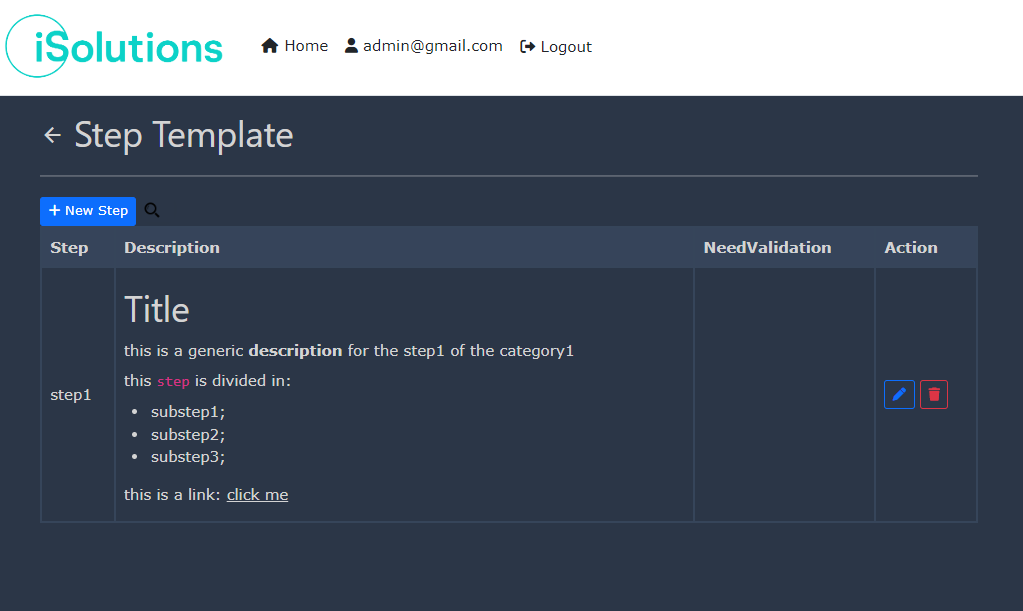
\includegraphics[width=0.9\textwidth]{img/markdown_pt2.png}
	\caption{esempio di visualizzazione in Markdown}
	\label{fig:markdown}
\end{figure}

Inoltre, per agevolare l'utilizzo di questa funzionalità, è stato incluso un apposito 
messaggio pop-up (figura~\ref{fig:markdownGuide}) che fornisce una semplice guida all'uso, completa di esempi pratici, 
al fine di consentire agli utenti di sfruttarla al meglio.

\begin{figure}[H]
	\centering
	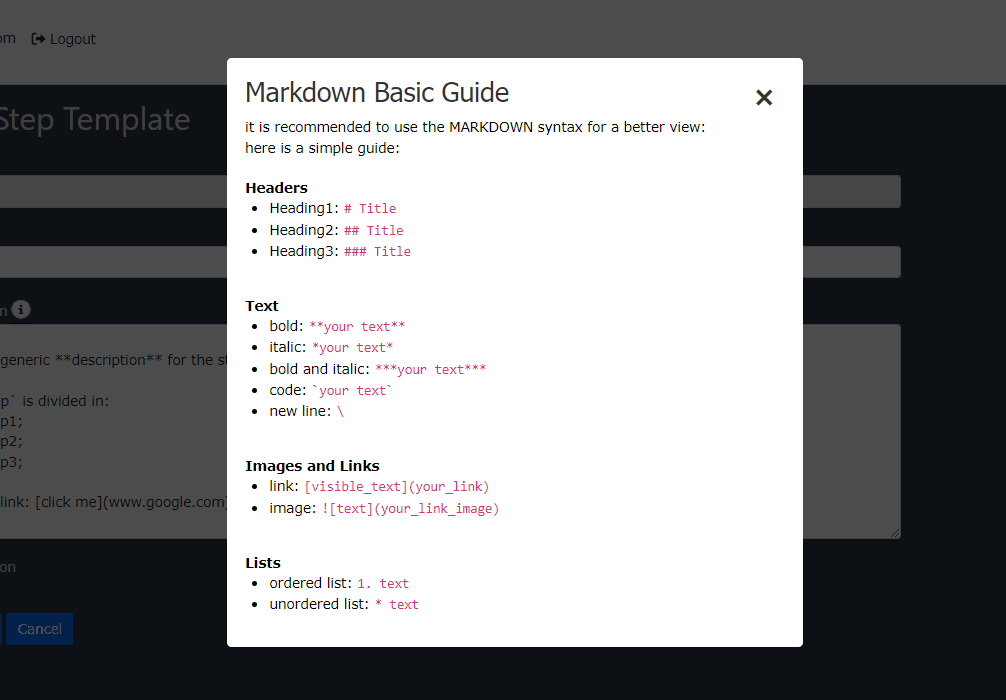
\includegraphics[width=0.9\textwidth]{img/markdownGuide1.png}
	\caption{guida basilare al Markdown}
	\label{fig:markdownGuide}
\end{figure}
\chapter{Il progetto e il suo sviluppo}\label{chapter:formattazione}
%
\section{Database}\label{sec:cap_sec_subsec}
Una parte sostanziale del lavoro impiegato per portare a compimento il
progetto si è concentrata in modo dettagliato sulla creazione del database,
ritenuto elemento cruciale per assicurare il pieno funzionamento della
piattaforma. \\ \\ La creazione del database è stata articolata in diverse fasi
chiave:
\begin{itemize}
	\item Progettazione della struttura del database, un processo attentamente studiato.
	\item Scrittura del database in linguaggio SQL, una tappa essenziale per l'implementazione della struttura.
	\item Implementazione delle interrogazioni al database nella sezione di backend,
	      facendo uso della libreria Dapper.
\end{itemize}
\textit{Nota}: il database è stato creato e gestito unicamente in locale per questioni di semplicità e per
l'esecuzione di test sulla correttezza della struttura e dell'implementazione del database stesso.
%
\subsection{Progettazione}
La fase di progettazione~\ref{fig:one} del database ha occupato un ruolo
fondamentale nel corso di questo processo, coinvolgendo un'analisi costante e
una riflessione profonda. L'obbiettivo principale è stato quello di plasmare un
database estremamente completo, in grado di soddisfare appieno le esigenze
della piattaforma di e-learning, ponendosi lo scopo aggiuntivo di:
\begin{itemize}
	\item Migliorare la leggibilità del database;
	\item Rendere più agevole la manutenzione;
	\item Fornire ampie possibilità di estensione del sistema.
\end{itemize}
\begin{figure}[ht]
	\centering
	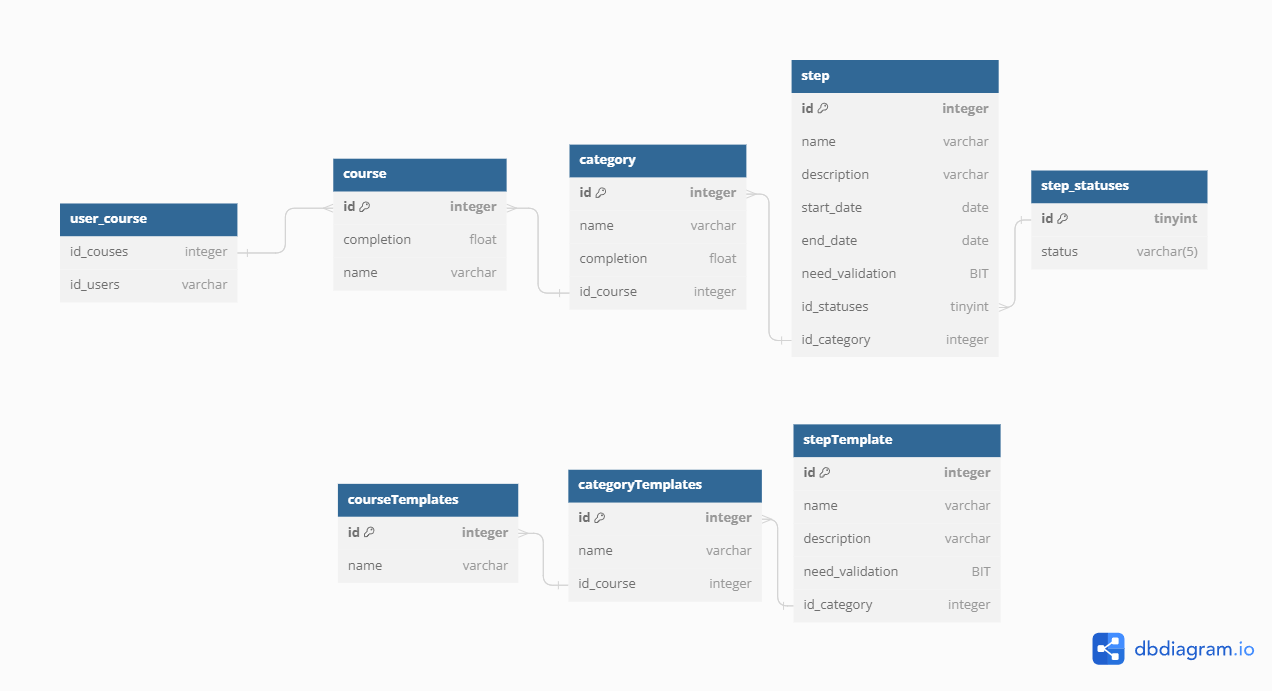
\includegraphics[width=1\textwidth]{img/progettazione_database.png}
	\caption{progettazione del database}
	\label{fig:one}
\end{figure}
\textit{Nota}: la progettazione mostrata non tiene traccia delle tabelle utente, perchè vengono
gestite automaticamente dal progetto .NET grazie al servizio di autenticazione già
incluso (libreria \inlinecode{Microsoft.AspNet.Identity.EntityFramework;}).
%
\\ \\
Si noti, inoltre, che non è stato creato un collegamento tra le tabelle “*Templates” con il resto del tabelle
perchè esse vengono gestite in maniera del tutto indipendente con le altre informazioni e relazioni presenti.
\begin{figure}[ht]
	\centering
	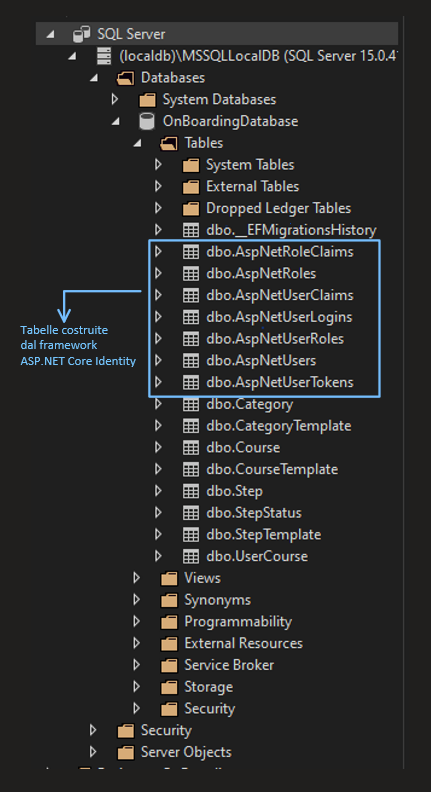
\includegraphics[width=0.5\textwidth]{img/TreeStructureDatabase.png}
	\caption{Tree structure del database}
	\label{fig:two}
\end{figure}
%
\subsection{Scrittura nel linguaggio SQL}
Il risultato finale di questa fase è il seguente~\ref{appendice-database} (non sono riportate le tabelle
generate dal servizio di Autenticazione, perchè gestite automaticamente dalla
libreria a disposizione)
%
\subsection{Interrogazioni al Database}
Inizialmente, le interrogazioni al database erano state sviluppate attraverso
\href{https://learn.microsoft.com/it-it/sql/relational-databases/stored-procedures/stored-procedures-database-engine?view=sql-server-ver16}{stored
	procedure}.\ Tra i numerosi vantaggi proposti, l'idea principale era ottenere:
\begin{itemize}
	\item Riutilizzo del codice;
	\item Semplificazione della manutenzione;
	\item Prestazioni migliorate;
\end{itemize}
Tuttavia, durante lo sviluppo dell'applicativo, grazie al suggerimento di alcuni membri
dell'azienda, si è preferito sostituire le procedure con interrogazioni dirette dal codice
tramite il framework \href{https://learn.microsoft.com/it-it/azure/azure-sql/database/elastic-scale-working-with-dapper?view=azuresql}{Dapper}, al fine di poter migliorare:
\begin{itemize}
	\item Prestazioni in termini di tempo;
	\item Semplificare il debugging del codice;
	\item Centrallizzare l'intera logica in un unico posto.
\end{itemize}
All'interno della piattaforma si possono distinguere 3 macro categorie di interrogazioni per:
\begin{itemize}
	\item Inserimento dei dati riguardanti:
		\begin{itemize}
			\item utenti
			\item corsi;
			\item categorie (sotto gruppo dei corsi);
			\item step (sotto gruppo delle categorie);
			\item corsi template;
			\item categorie template (sotto gruppo dei corsi template);
			\item step template (sotto gruppo delle categorie template).
		\end{itemize}
	\item Eliminazione dei dati riguardanti:
		\begin{itemize}
			\item utenti
			\item corsi;
			\item categorie (sotto gruppo dei corsi);
			\item step (sotto gruppo delle categorie);
			\item corsi template;
			\item categorie template (sotto gruppo dei corsi template);
			\item step template (sotto gruppo delle categorie template).
		\end{itemize}
	\item Lettura dei dati per permettere di ottenere tutte le informazioni necessarie
		per la generazione corretta della pagina dinamica dato un determinato utente
		connesso;
\end{itemize}
%
\section{Scrittura del codice C\#}\label{sec:cap_sec_subsec}
La parte del codice back-end rappresenta il nucleo vitale dell'intero progetto, 
che ne garantisce il corretto funzionamento. Questa componente è stata completamente 
sviluppata utilizzando il linguaggio di programmazione C\#.
\\ \\
L'obbiettivo principale è stato garantire una gestione efficiente del database
direttamente attraverso il codice, sfruttando appieno le potenzialità del
framework Dapper. \\ 
Utilizzando C\# e il framework Dapper, è stato possibile
realizzare un corretto collegamento tra dati e utenti.\ Questo ha reso
possibile la generazione dinamica e accurata delle pagine web, consentendo
un'esperienza utente ottimale. 
\\ \\ 
Per eseguire delle query al database è
stato necessario creare una connessione dal codice C\# al database attraverso
la libreria \inlinecode{Microsoft.Data.SqlClient;}
%
%TODO: fixhere
\begin{algorithm}[H]
	\caption{classe per ottenere la stringa di connessione per il collegamento al database}
	\label{lst:genic_mpi}
	\begin{lstlisting}[label=lst:test]
using Microsoft.Data.SqlClient;
using Microsoft.EntityFrameworkCore;

namespace OnBoarding.Services
{
	public class ConnectionService
	private SqlConnection _connection = new SqlConnection();
	private SqlCommand _command = new SqlCommand();

	public static IConfiguration? Configuration { get; set; }

	public string GetconnectionString()
	{
		var builder = new ConfigurationBuilder().SetBasePath(Directory.GetCurrentDirectory()).AddJsonFile("appsettings.json");

		Configuration = builder.Build();
		return Configuration.GetConnectionString("ApplicationDBContextConnection");
	}


	public SqlConnection GetConnection() 
	{
		return _connection;
	}

	public SqlCommand GetCommand()
	{
		return _command;
	}

	}
}
	\end{lstlisting}
\end{algorithm}
%
In questo modo, una volta che è stata stabilita una connessione, 
è stato reso possibile il processo di scrittura di query. A titolo esemplificativo, si può menzionare 
la query nella funzione denominata ``GetCourses'' presente all'interno del file ``CourseManager.cs''.\ Questa query, 
quando viene fornito l'ID dell'utente come input, ha lo scopo principale di recuperare e restituire 
l'insieme completo dei corsi associati all'utente specificato.
%
%TODO: fixhere
\begin{algorithm}[H]
	\caption{esempio funzione per l'esecuzione di una query da codice tramite il framework Dapper}
	\label{lst:genic_mpi}
	\begin{lstlisting}[label=lst:test]
public List<CourseModel> GetCourses(string userid)
{
	using (_connection = new SqlConnection(connectionService.GetconnectionString()))
	{
		_connection.Open();

		string sql = 
			@"SELECT DISTINCT Course.* 
			FROM Course, AspNetUsers, UserCourse 
			WHERE UserCourse.UserId = @userId     
			AND UserCourse.CourseId = Course.Id";
		var coursesList = _connection.Query<CourseModel>(sql, new { userId = userid }).ToList();

		_connection.Close();

		return coursesList;
	}
} 
	\end{lstlisting}
\end{algorithm}
%
Si osserva che ciascun utente può essere associato a più corsi, 
stabilendo così una relazione uno a molti.\ Pertanto, è fondamentale 
che il valore restituito dalla funzione sia di tipo \inlinecode{List\textless CourseModel \textgreater}, 
in quanto questa struttura dati può contenere più di un corso associato a 
un utente specifico.\ Inoltre, grazie all'uso di Dapper, è possibile effettuare 
un'interrogazione al database mediante una stringa appositamente creata 
(come mostrato nelle righe 7\--11 del codice).\ Successivamente, è possibile 
ottenere il risultato dell'interrogazione corrispondente al parametro ``userid'' 
fornito alla funzione e al campo ``userId'' nella tabella ``Course'' (riga 12 del codice).
\\
Notare che siccome la funzione ritorna in questo caso una lista, il risultato della query
dovrà essere convertito in una collezione di oggetti dello stesso tipo (attraverso alla funzione \inlinecode{ToList()}).
%
\\ \\
%
Un punto di particolare rilevanza che merita menzione è rappresentato dallo sviluppo di una classe denominata 
``StatisticsController.cs''.\ Il suo scopo principale consiste nell'elaborare in modo esaustivo e dettagliato tutte 
le statistiche associate a un utente specifico.\ Questa classe si avvale della sofisticata libreria \inlinecode{ClosedXML.Excel;} 
per generare dati statistici inerenti al completamento dei corsi che sono stati non solo avviati, ma anche portati a 
termine dall'utente in questione.\ È essenziale sottolineare che questa funzionalità è rigorosamente riservata agli 
utenti che detengono il privilegiato ruolo di ``Admin''.
% TODO: add image
%
% TODO: fixhere
% \begin{algorithm}[H]
% 	\caption{esempio funzione per l'esecuzione di una query da codice tramite il framework Dapper}
% 	\label{lst:genic_mpi}
% 	\begin{lstlisting}[label=lst:test]
% [HttpGet]
% [Authorize(Roles = "Admin")]
% public IActionResult ExportToExcel(int id)
% {
% 	using (var workbook = new XLWorkbook())
% 	{
% 		CourseModel course = _courseManager.GetCourseByID(id);

% 		var ws = workbook.Worksheets.Add(course.Name); // Sheet Name
% 		int i = 1;

% 		/////////////////////////////////////// Course
% 		ws.Range($"A{i}:E{i}").Merge();
% 		ws.Cell(i, 1).Value = "Course";
% 		ws.Cell(i, 1).Style.Font.Bold = true;
% 		ws.Cell(i, 1).Style.Alignment.Horizontal = XLAlignmentHorizontalValues.Center;
% 		ws.Cell(i, 1).Style.Font.FontSize = 30;

% 		// Header
% 		i++;
% 		ws.Cell(i, 1).Value = "Id";
% 		ws.Cell(i, 2).Value = "Name";
% 		ws.Cell(i, 3).Value = "Completion";
% 		ws.Cell(i, 4).Value = "StartDate";
% 		ws.Cell(i, 5).Value = "EndDate";
% 		ws.Range($"A{i}:E{i}").Style.Fill.BackgroundColor = XLColor.Alizarin;

% 		// Body
% 		i++;
% 		ws.Cell(i, 1).Value = course.Id;
% 		ws.Cell(i, 2).Value = course.Name;
% 		ws.Cell(i, 3).Value = course.Completion;
% 		if (course.StartDate != DateTime.MinValue) ws.Cell(i, 4).Value = course.StartDate.ToString();
% 		else { ws.Cell(i, 4).Value = "NULL"; ws.Cell(i, 4).Style.Font.FontColor = XLColor.Red; }
% 		if (course.EndDate != DateTime.MinValue) ws.Cell(i, 5).Value = course.EndDate.ToString();
% 		else { ws.Cell(i, 5).Value = "NULL"; ws.Cell(i, 5).Style.Font.FontColor = XLColor.Red; }
% 		ws.Range($"A{i}:E{i}").Style.Fill.BackgroundColor = XLColor.AliceBlue;
% 		i += 1;

% 		// ...
% 		// Stesso procedimento appena descritto per i Corsi, viene fatto
% 		// per le Categorie e gli Step 
%		
% 		using (var stream = new MemoryStream())
% 		{
% 			workbook.SaveAs(stream);
% 			var content = stream.ToArray();
% 			return File(
% 					content,
% 					"application/vnd.openxmlformats-officedocument-spreadsheetml.sheet",
% 					course.Name + ".csv"
% 				);
% 		}
% 	}
% }
% 	\end{lstlisting}
% \end{algorithm}
%
Un aspetto di notevole rilevanza è stato il processo di gestione dei dati statistici all'interno della pagina denominata 
``/Views/Statistics/Index.cshtml''.\ Questa pagina ha una funzione fondamentale poiché consente agli admin di visualizzare 
l'insieme completo delle statistiche.\ Ciò è reso possibile grazie alla capacità di ordinare agevolmente le informazioni 
presenti all'interno delle tabelle.\ Questa caratteristica permette agli utenti di organizzare i dati in base alle loro 
specifiche esigenze e criteri di ricerca.
\\
Inoltre, per rendere l'esperienza ancora più interattiva e informativa, è stata inclusa una sezione di codice dedicata 
direttamente all'interno della pagina stessa, utilizzando il tag \inlinecode{<script>\dots</script>}. Questo approccio ha 
consentito di incorporare efficacemente dei grafici che offrono una rappresentazione visiva dei dati statistici.\ 
Questi grafici sono stati sviluppati in modo da offrire quattro diverse visualizzazioni, ognuna delle quali fornisce un'analisi 
dettagliata dei dati statistici, permettendo agli utenti di comprendere meglio i pattern e le tendenze sottostanti.
\begin{itemize}
	\item due grafici a barre;
	\begin{itemize}
		\item Il primo rappresenta la somma totale dei corsi suddivisi per stato di completamento (done, running, todo);
		\item Il secondo rappresenta il numero di corsi completati in relazione al mese dell'anno.
	\end{itemize}
	\item due grafici a torta;
	\begin{itemize}
		\item Il primo rappresenta il tempo medio di completamento necessario per terminare uno specifico corso, suddiviso per corso;
		\item Il secondo rappresenta il tempo medio di completamento necessario per teminare uno specifico corso, suddiviso per utenti.
	\end{itemize}
\end{itemize}
L'implementazione del codice per la creazione dei grafici è stata effettuata mediante l'uso del linguaggio di programmazione JavaScript.\ 
Un aspetto interessante da sottolineare è che i dati numerici necessari per la creazione dei grafici non sono stati ottenuti direttamente 
tramite il codice JavaScript, ma sono stati acquisiti attraverso apposite funzioni getter scritte in codice C\#.\ 
Questo approccio è stato adottato per garantire l'accuratezza e la coerenza dei dati, nonché per sfruttare le funzionalità di gestione 
dei dati messe a disposizione dal linguaggio C\#.\
In sostanza, il processo è stato il seguente: il codice JavaScript si è interfacciato con il codice C\# attraverso apposite funzioni getter, 
ottenendo così i dati numerici necessari per alimentare i grafici.\
% TODO: fix
\begin{algorithm}[H]
 	\caption{esempio sezione codice Javascript per la creazione di un grafico a barre per la rappresentazione dei dati}
 	\label{lst:genic_mpi}
 	\begin{lstlisting}[label=lst:test]
<script>
	// ...
	
	/*-------------------------------- BAR CHART --------------------------------*/
    var xValues = ["To Do", "Running", "Done"];
    var yValues = [@todo, @running, @done, 0];
    var barColors = ["red", "#e5e600", "green"];

    new Chart("BarChart", {
        type: "bar",
        data: {
            labels: xValues,
            datasets: [{
                backgroundColor: barColors,
                data: yValues
            }]
        },
        options: {
            legend: { display: false },
            title: {
                display: false,
                text: ""
            }
        }
    });

	// ...
</script>
 	\end{lstlisting}
\end{algorithm}
% TODO: add image
%
\section{Layout della piattaforma}\label{sec:cap_sec_subsec}
Il layout della piattaforma è stato attentamente progettato e realizzato con l'obiettivo di 
creare un servizio che sia estremamente intuitivo e facile da utilizzare, sia per gli utenti 
che per gli amministratori responsabili della gestione degli accessi e del progresso degli utenti 
durante il loro percorso nell'esperienza.\ Grazie a questa attenzione al design e all'usabilità, 
è stato possibile assicurarsi che l'intera esperienza sia accessibile e fruibile in modo agevole 
e soddisfacente per tutti i suoi utilizzatori.
\chapter{Risultati e sviluppi futuri}\label{chapter:formattazione}
%
%
\section{Risultati}\label{sec:cap_sec_subsec}
%
%* TODO: ADD INFO 
%
\section{Sviluppi fututi}\label{sec:cap_sec_subsec}
\subsection{Pagina statistiche}\label{sec:cap_sec_subsec}
La pagina delle statistiche deve subire un notevole potenziamento, mirando a offrire un'esperienza più completa ed esaustiva.\ 
Questo miglioramento deve concentrarsi sulla possibilità di confrontare una quantità più ampia di dati, 
garantendo al contempo un maggiore spazio dedicato all'analisi dei dati.\ 
Questa evoluzione si rivolge in particolare al personale del reparto HR dell'azienda, 
che ha la responsabilità di gestire il processo di OnBoarding per una varietà di utenti.
\\ \\
Grazie alla capacità di consentire un confronto più dettagliato dei dati, questa pagina deve diventare uno strumento prezioso per l'HR.\ 
Inoltre, dovrebbe essere possibile implementare un numero maggiore di grafici interattivi, che contribuiranno significativamente 
alla comprensione e all'analisi dei dati.
\\ \\
Questo potenziamento non solo agevolerà il processo decisionale dell'HR, ma permetterà anche di individuare con precisione le aree 
che richiedono interventi e miglioramenti.\ In definitiva, mira a trasformare la pagina delle statistiche in uno strumento 
fondamentale per l'ottimizzazione dell'OnBoarding all'interno del contesto dell'azienda.
%
\subsection{Ruoli utente}\label{sec:cap_sec_subsec}
Un'ulteriore evoluzione e arricchimento del sistema potrebbe senz'altro consistere nell'espandere 
l'attuale struttura dei ruoli, che attualmente comprende solo due categorie: ``User'' e ``Admin''.\ 
Questa espansione comporterebbe l'aggiunta di ulteriori ruoli, consentendo così una maggiore granularità nei 
permessi di visualizzazione all'interno delle pagine generate.
\\ \\  
L'implementazione di ruoli aggiuntivi potrebbe essere estremamente vantaggiosa, poiché permetterebbe di adattare 
l'accesso alle informazioni in base alle specifiche responsabilità e autorizzazioni di ciascun utente.\ 
In questo modo, si potrebbe garantire un maggiore controllo sull'accesso ai dati sensibili e una gestione 
più efficiente delle risorse aziendali.
\\ \\
Questo approccio fornirebbe ai decision-maker una maggiore flessibilità nella configurazione dei permessi e consentirebbe 
di assegnare ruoli intermedi, ad esempio ``Supervisor'' o ``Manager'', con diritti di accesso mirati alle informazioni rilevanti 
per il loro ruolo.\ Ciò migliorerebbe la sicurezza dei dati e l'efficienza operativa, 
consentendo a ciascun membro del team di accedere solo alle risorse necessarie per svolgere le proprie mansioni.
%
\subsection{Creazione dei Corsi}\label{sec:cap_sec_subsec}
Un aspetto che potrebbe essere considerato di importanza secondaria, ma che indubbiamente contribuirebbe al miglioramento 
significativo dell'esperienza utente, soprattutto dal punto di vista dell'amministratore, 
riguarda la possibilità di creare Corsi o CorsiTemplate in modo più efficiente, attraverso l'utilizzo di un nuovo processo/i di creazione.\ 
Attualmente, questa operazione richiede un processo manuale, ma esistono alternative 
che potrebbero semplificarne notevolmente l'implementazione.
\\ \\
Una di queste opzioni sarebbe consentire agli amministratori di importare direttamente i dati relativi ai Corsi o ai CorsiTemplate 
da fogli Excel.\ Questo approccio eliminerebbe gran parte del lavoro manuale, 
consentendo di caricare rapidamente una quantità significativa di informazioni nel sistema.
\\ \\
Inoltre, potrebbe essere utile considerare l'integrazione di funzionalità native all'interno del sito web per la creazione 
di Corsi o CorsiTemplate.\ Queste funzionalità integrate potrebbero offrire un ambiente più intuitivo e user-friendly 
per la progettazione e la gestione dei Corsi, migliorando ulteriormente l'esperienza dell'amministratore.
\\ \\
In definitiva, anche se questa caratteristica potrebbe essere considerata di importanza secondaria, 
l'implementazione di strumenti per l'importazione da Excel o funzionalità native all'interno del sito 
rappresenterebbe un passo avanti significativo nella semplificazione delle attività legate alla creazione di Corsi e CorsiTemplate, 
contribuendo in modo tangibile all'efficienza operativa complessiva e al miglioramento dell'esperienza dell'utente amministratore. 
\\ \\
\textit{Nota: } attualmente l'unica modalità per la creazione di nuovi Corsi e CorsiTemplate completi di relative Categorie e Step è la seguente:
\begin{enumerate}
    \item creazione del corso;
    \item apertura del corso;
    \item creazione della categoria;
    \item apertura della categoria;
    \item creazione dello step;
\end{enumerate}
%
\subsection{Text editor}\label{sec:cap_sec_subsec}
Attualmente, la feature che consente la scrittura in sintassi Markdown è piuttosto limitata e semplice.\
Potrebbe essere opportuno valutare l'implementazione di un vero e proprio editor di testo dedicato, 
in aggiunta alla possibilità di scrivere il Markdown manualmente.\ Questa aggiunta consentirebbe agli 
utenti di sfruttare gli stili di formattazione e i vantaggi offerti dalla sintassi Markdown in modo molto più facile, 
inclusivo ed intuitivo per tutti.\ Grazie alla presenza di appositi tasti funzione e a un ambiente di scrittura 
appositamente progettato, si potrebbero sfruttare al meglio tutte le potenzialità della formattazione Markdown 
senza la necessità di conoscere a fondo la sua sintassi.\ Questo migliorerebbe notevolmente l'esperienza degli 
utenti e renderebbe l'utilizzo di questa funzionalità ancora più accessibile e versatile.
\\
Di seguito un esempio preso dal programma ``Slack'':
\begin{figure}[ht]
	\centering
	
\includegraphics[width=1\textwidth]{img/textEditor.png}
	\caption{esempio di un possibile text editor}
	\label{fig:one}
\end{figure}
%
%
\subsection{Reportistica errori e commenti}\label{sec:cap_sec_subsec}
\subsubsection{Reportistica errori}
Una possibile feature futura che potrebbe rivelarsi estremamente utile riguarderebbe 
l'integrazione di un meccanismo avanzato che consenta agli utenti incaricati di svolgere 
i corsi all'interno della piattaforma di segnalare errori o imprecisioni nei task assegnati.\ 
Questa innovativa funzionalità darebbe agli utenti la preziosa possibilità di comunicare direttamente 
agli amministratori eventuali problemi o lacune, come ad esempio link non funzionanti dovuti a modifiche 
nel corso del tempo o informazioni errate nelle assegnazioni.\ Inoltre, potrebbe includere anche la segnalazione 
di descrizioni mancanti o insufficientemente complete, offrendo un quadro completo delle aree da migliorare.
\\ \\
L'introduzione di questa avanzata funzionalità consentirebbe agli amministratori di ricevere feedback costanti 
da parte degli utenti, contribuendo così in modo significativo a elevare la qualità del servizio offerto.\ 
Inoltre, fornirebbe un meccanismo efficace per mantenere sempre aggiornati e corretti i contenuti presenti 
sulla piattaforma, garantendo agli utenti una esperienza di apprendimento completa e senza interruzioni.
\subsubsection{Commenti}
Potrebbe rivelarsi di di grande utilità considerare l'aggiunta di un sistema di assistenza diretta agli utenti 
tramite appositi commenti, in modo che gli utenti possano richiedere aiuto agli amministratori in maniera immediata.\ 
Sistema che potrebbe essere implementato in modo da consentire la comunicazione in threads dedicati, dove 
ogni nuovo messaggio può essere gestito in modo organizzato e pertinente.\ 
Questa funzionalità potrebbe essere integrata insieme alla feature di segnalazione degli errori o essere 
inserita in una sezione separata, per garantire un supporto completo e altamente efficiente per tutti gli utenti finali, 
migliorando notevolmente l'esperienza globale sulla piattaforma.
%
\subsection{Layout della piattaforma}\label{sec:cap_sec_subsec}
Attualmente, il layout della piattaforma si presenta con un design estremamente minimalista, 
concentrandosi esclusivamente su ciò che è strettamente necessario per la corretta visualizzazione 
dei dati e delle informazioni presenti nella piattaforma.\ Questo stile, sebbene efficiente, 
può essere considerato non particolarmente moderno.\ Pertanto, una delle possibili migliorie potrebbe 
consistere nell'apportare alcune modifiche significative al layout stesso, con l'obiettivo di migliorare l'esperienza dell'utente.
\\ \\
Una proposta consisterebbe nell'introduzione di navbar più complete e informative, specialmente per gli amministratori.\ 
Queste navbar potrebbero offrire un accesso rapido alle funzionalità e agli strumenti di amministrazione, 
semplificando così le attività di gestione e supervisione dell'intero sistema.
\\ \\
Inoltre, potrebbe essere benefico considerare l'implementazione di specifiche side-navbar per gli utenti, 
soprattutto quando si trovano nella pagina di visualizzazione dei corsi.\ 
Attualmente, la ricerca di task specifici da completare all'interno di un corso potrebbe risultare disorientante per l'utente finale, 
in quanto potrebbe richiedere uno sforzo eccessivo per individuare le informazioni rilevanti.\ 
L'aggiunta di una side-navbar dedicata potrebbe semplificare notevolmente questa operazione, 
consentendo agli utenti di accedere rapidamente ai alle categorie o ai task all'interno del corso senza difficoltà.
\\ \\
In conclusione, apportare modifiche al layout della piattaforma attraverso l'implementazione di navbar 
più esaustive per gli admin e di side-navbar specifiche per gli utenti, soprattutto nella pagina di visualizzazione dei corsi, 
rappresenterebbe un passo importante per migliorare l'usabilità complessiva del sistema e l'esperienza dell'utente finale.
%

%
%
%%%% Le Conclusioni
\pagestyle{plain}
\chapter*{Conclusione} %Se si cambia il Titolo cambiare anche la riga successiva così che appia corretto nell'conclusione
\addcontentsline{toc}{chapter}{Conclusione} %Per far apparire Introduzione nell'indice (Il nome deve rispecchiare quello del chapter)
%
In conclusione, durante il mio tirocinio, ho sviluppato un'applicazione web basata su .NET MVC 6.0 con 
l'obiettivo di creare un servizio che automatizzasse in modo efficiente il 
processo di integrazione dei nuovi dipendenti, un passaggio cruciale e ricorrente per 
tutti i nuovi membri dell'organico aziendale.\ Questo progetto ha consentito 
all'azienda di mettere a disposizione uno strumento estremamente automatizzato, riducendo 
significativamente il carico di lavoro del dipartimento HR e delegando gran parte delle 
attività operative alla gestione automatizzata del sistema.
\\ \\ 
In particolare, il tempo di gestione del processo di Onboarding da parte del reparto HR  è il seguente:
%TODO: fix position
\begin{figure}
	\centering
	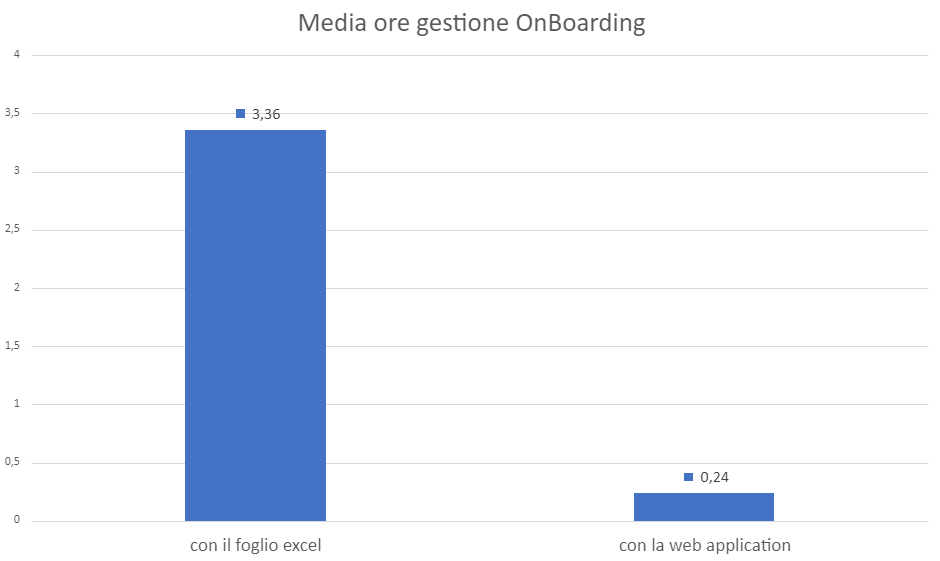
\includegraphics[width=\textwidth]{img/conclusione1.png}
	\label{fig:conclusione1}
	\caption[media ore di gestione del processo di OnBoarding]{Nel grafico visualizzato, vengono considerati esclusivamente i periodi di tempo dedicati dal personale 
	del dipartimento HR alla coordinazione del processo Onboarding durante il suo ciclo per un utente specifico. I dati 
	temporali riportati sono calcolati come una media basata sui tre OnBoarding più recenti gestiti.
	È importante sottolineare che le informazioni fornite nel grafico non riflettono la durata complessiva del processo, 
	bensì rappresentano unicamente il tempo impiegato dal personale HR per garantirne una corretta gestione.}
\end{figure}

Va notato che l'azienda, in virtù della sua certificazione ISO 9001, non solo è obbligata a farlo, 
ma si impegna attivamente a gestire e analizzare attentamente i feedback provenienti dagli utenti del sistema, 
con l'obiettivo di migliorarne costantemente l'efficacia e l'efficienza.
\\ \\
L'applicazione web, pur rispettando appieno tutti i requisiti aziendali iniziali, 
offre un ampio margine per ulteriori miglioramenti, come discusso dettagliatamente nel capitolo dedicato del documento~\ref{chapter:Risultati_e_sviluppi_futuri}, 
offrendo così opportunità significative per un futuro sviluppo e ottimizzazione.
%
%%%% La bibliografia
% \bibliographystyle{apalike} %{plain} -- Scegliere lo stile preferito
% \cleardoublepage
% \addcontentsline{toc}{chapter}{\bibname}
%\bibliography{./Bibliografia}
%
\chapter*{Ringraziamenti}
Desidero ringraziare sinceramente le seguenti persone dell'azienda ISolutions che mi hanno 
accompagnato e guidato durante l'esecuzione del mio progetto di tirocinio:
\begin{itemize}
    \item Alessandro Bardini (Line Manager) \& Gialuca Bellini (Line Manager \-- NOC Team Lead).\ Per la loro preziosa guida nell'ambito dell'esecuzione dei vari compiti del progetto.
    \item Ivan Anselmi (Architect, R\&D Dev).\ Per l'assistenza nell'applicazione del servizio di Autenticazione, per la guida su come implementare al meglio il framework Dapper e per i consigli e le linee guida forniti per ottenere la corretta gestione delle query string nella realizzazione della piattaforma web sviluppata.
    \item Roberto Isca (Senior Web Designer \& Web Developer).\ Per i preziosi consigli e l'aiuto fornito in numerosi problemi di layout.
    \item Marco Chiesa (System Engineer).\ Per aver reso possibile il mio lavoro in remoto grazie alla configurazione della VPN e dei servizi aziendali.
\end{itemize}
%
Ringrazio, inoltre, coloro che mi hanno fornito preziosi consigli e che mi hanno sostenuto sia durante il progetto di tirocinio sia nella stesura di questo elaborato:
\begin{itemize}
    \item Donatello Larocca.
    \item Mariachiara Michelini.
\end{itemize}
%
Il loro sostegno e la loro guida sono stati fondamentali.\ Grazie di cuore a tutti loro.
%
% Le appendici
\appendix
\chapter{Scrittura del Database}
%
\label{appendice-database}
\begin{lstlisting}[style=sql_style, caption=tabelle per la creazione del database utilizzato]
CREATE TABLE [dbo].[Course] ( 
    [Id]         INT            IDENTITY (1, 1) NOT NULL, 
    [Name]       NVARCHAR (255) NOT NULL, 
    [Completion] REAL           DEFAULT ((0)) NULL, 
    [StartDate]  DATETIME2 (7)  NULL, 
    [EndDate]    DATETIME2 (7)  NULL, 
    CONSTRAINT [PK_Course] PRIMARY KEY CLUSTERED ([Id] ASC) 
); 

CREATE TABLE [dbo].[Category] ( 
    [Id]         INT            IDENTITY (1, 1) NOT NULL, 
    [Name]       NVARCHAR (255) NOT NULL, 
    [Completion] REAL           DEFAULT ((0)) NULL, 
    [IdCourse]   INT            NOT NULL, 
    CONSTRAINT [PK_Category] PRIMARY KEY CLUSTERED ([Id] ASC), 
    CONSTRAINT [FK_Category_Course_IdCourse]
    FOREIGN KEY ([IdCourse]) REFERENCES [dbo].[Course] ([Id]) 
    ON DELETE CASCADE 
    ); 
    GO 
    CREATE NONCLUSTERED INDEX [IX_Category_IdCourse] 
        ON [dbo].[Category]([IdCourse] ASC); 	

-- 3 stati: 
    -- 1. done 
    -- 2. todo 
    -- 3. check 
CREATE TABLE [dbo].[StepStatus] ( 
    [Id]     INT            IDENTITY (1, 1) NOT NULL, 
    [Status] NVARCHAR (10) NOT NULL, 
    CONSTRAINT [PK_StepStatus] PRIMARY KEY CLUSTERED ([Id] ASC) 
); 

CREATE TABLE [dbo].[Step] ( 
    [Id]             INT            IDENTITY (1, 1) NOT NULL, 
    [Name]           NVARCHAR (255) NOT NULL, 
    [Description]    NVARCHAR (MAX) NULL, 
    [StartDate]      DATETIME2 (7)  NULL, 
    [EndDate]        DATETIME2 (7)  NULL, 
    [Lock]           BIT            DEFAULT ((1)) NULL, 
    [NeedValidation] BIT            DEFAULT ((0)) NULL, 
    [IdStatus]       INT            DEFAULT ((1)) NULL, 
    [IdCategory]     INT            NOT NULL, 
    CONSTRAINT [PK_Step] PRIMARY KEY CLUSTERED ([Id] ASC), 
    CONSTRAINT [FK_Step_StepStatus_IdStatus]  
FOREIGN KEY ([IdStatus]) REFERENCES [dbo].[StepStatus] ([Id]) 
ON DELETE CASCADE, 
    CONSTRAINT [FK_Step_Category_IdCategory]  
FOREIGN KEY ([IdCategory]) REFERENCES [dbo].[Category] ([Id]) 
ON DELETE CASCADE 
); 
GO 
CREATE NONCLUSTERED INDEX [IX_Step_IdCategory] 
    ON [dbo].[Step]([IdCategory] ASC); 
GO 
CREATE NONCLUSTERED INDEX [IX_Step_IdStatus] 
    ON [dbo].[Step]([IdStatus] ASC); 

CREATE TABLE [dbo].[UserCourse] ( 
    [UserId]   NVARCHAR (450) NOT NULL, 
    [CourseId] INT            NOT NULL, 
    CONSTRAINT [FK_UserCourse_Course_CourseModel]  
FOREIGN KEY ([CourseId]) REFERENCES [dbo].[Course] ([Id]) 
ON DELETE CASCADE, 
    CONSTRAINT [FK_UserCourse_AspNetUsers_UserId]  
FOREIGN KEY ([UserId]) REFERENCES [dbo].[AspNetUsers] ([Id]) 
ON DELETE CASCADE 
); 
GO 
CREATE NONCLUSTERED INDEX [IX_UserCourse_CourseModel] 
    ON [dbo].[UserCourse]([CourseId] ASC); 
GO 
CREATE NONCLUSTERED INDEX [IX_UserCourse_UserId] 
    ON [dbo].[UserCourse]([UserId] ASC); 
    
CREATE TABLE [dbo].[CourseTemplate] ( 
    [Id]             INT            IDENTITY (1, 1) NOT NULL, 
    [Name]           NVARCHAR (255) NOT NULL, 
    [Creator]        NVARCHAR (255) NOT NULL, 
    [CreationDate]   DATETIME2 (7)  NULL, 
    [LastUpdateDate] DATETIME2 (7)  NULL, 
    CONSTRAINT [PK_CourseTemplate] PRIMARY KEY CLUSTERED ([Id] ASC) 
); 
    
CREATE TABLE [dbo].[CategoryTemplate] ( 
    [Id]                INT         IDENTITY (1, 1) NOT NULL, 
    [name]              NCHAR (255) NOT NULL, 
    IDCourseTemplate INT         NOT NULL, 
    PRIMARY KEY CLUSTERED ([Id] ASC), 
    FOREIGN KEY (IDCourseTemplate)  
    REFERENCES [dbo].[CourseTemplate] ([Id]) 
    ON DELETE CASCADE 
); 
    
CREATE TABLE [dbo].[StepTemplate] ( 
    [Id]                 INT            IDENTITY (1, 1) NOT NULL, 
    [Name]               NVARCHAR (255) NOT NULL, 
    [Description]        NVARCHAR (MAX) NOT NULL, 
    [NeedValidation]     BIT            DEFAULT ((0)) NULL, 
    [IDCategoryTemplate] INT            NOT NULL, 
    CONSTRAINT [PK_StepTemplate] PRIMARY KEY CLUSTERED ([Id] ASC), 
    CONSTRAINT [FK_StepTemplate_CategoryTemplate_IDCategoryTemplate]  
    FOREIGN KEY ([IDCategoryTemplate]) REFERENCES [dbo].[CategoryTemplate] ([Id]) 
    ON DELETE CASCADE 
); 
GO 
CREATE NONCLUSTERED INDEX [IX_StepTemplate_IDCategoryTemplate] 
    ON [dbo].[StepTemplate]([IDCategoryTemplate] ASC);
\end{lstlisting}
%
\end{document}